\clearpage
\onecolumn
\setcounter{section}{0}
\renewcommand{\thesection}{\Alph{section}}
\maketitlesupplementary

% Table of Contents
\section*{Table of Contents}
\startcontents[appendices]
\printcontents[appendices]{l}{1}{\setcounter{tocdepth}{3}}

\clearpage

%% ============================================================
%% §A  The E-Deflare Benchmark in Detail
%% ============================================================

\section{The E-Deflare Benchmark in Detail}
\label{app:benchmark_details}

\subsection{E-Flare2.7K: Simulated Dataset}
\label{app:eflare_details}

The \textbf{E-Flare2.7K} dataset is constructed using our physics-driven simulator, fusing dynamic simulated flare events with real-world background events via the PNL-ES operator, ensuring physically grounded interaction rather than simple linear addition.

\noindent\textbf{Background Event Scenes.}
Background events ($\mathbf{E}_{\mathrm{bg}}$) are sampled from the DSEC dataset~\cite{gehrig2021dsec}. We utilize seven distinct long-duration sequences capturing diverse urban driving environments (\eg, \texttt{zurich\_city\_00\_a}, \texttt{interlaken\_00\_c}). For each training sample, a random temporal window of $50$--$100$~ms is extracted, providing rich variety in motion patterns and event densities.

\noindent\textbf{Flare Event Generation.}
A deterministic script-based synchronization strategy ensures perfect spatio-temporal alignment between $\mathbf{E}_{\textcolor{ev_red}{\mathrm{\mathbf{f}}}}$ and $\mathbf{E}_{\mathrm{light}}$. Key aspects include:
\begin{itemize}
    \item \textbf{Source Assets:} Paired static assets from Flare7K++~\cite{dai2024flare7k++}, covering scattering and reflective flare types.
    \item \textbf{Motion Profiles:} Smooth linear trajectories with random start positions, directions ($0$--$360$°), and travel distances (up to $180$ pixels).
    \item \textbf{Geometric Augmentations:} Random rotations ($0$--$360$°), scaling ($0.8$--$1.5\times$), translations ($\pm20$\%), and shearing ($\pm20$°).
    \item \textbf{Intensity Flicker:} Periodic flickering at $100$--$140$~Hz with varied waveforms (sine, square, triangle); stable (non-flickering) sources simulated in $30\%$ of samples.
    \item \textbf{Hybrid Flare Rendering:} Scattering flare animated from Flare7K++ assets; reflective flare synthesized via a custom real-time shader pipeline applied in $90\%$ of sequences (to be released with code).
    \item \textbf{Event Generation:} Videos rendered at up to $6{,}000$~FPS and converted to event streams via DVS-Voltmeter~\cite{lin2022dvs} with randomized contrast thresholds.
\end{itemize}
The resulting dataset contains $\mathbf{2{,}720}$ paired $20$~ms samples at $640 \times 480$, split into $\mathbf{2{,}545}$ for training and $\mathbf{175}$ for testing. Representative samples are shown in Fig.~\ref{APfig:dataset_eflare}.

\begin{figure}[H]
    \centering
    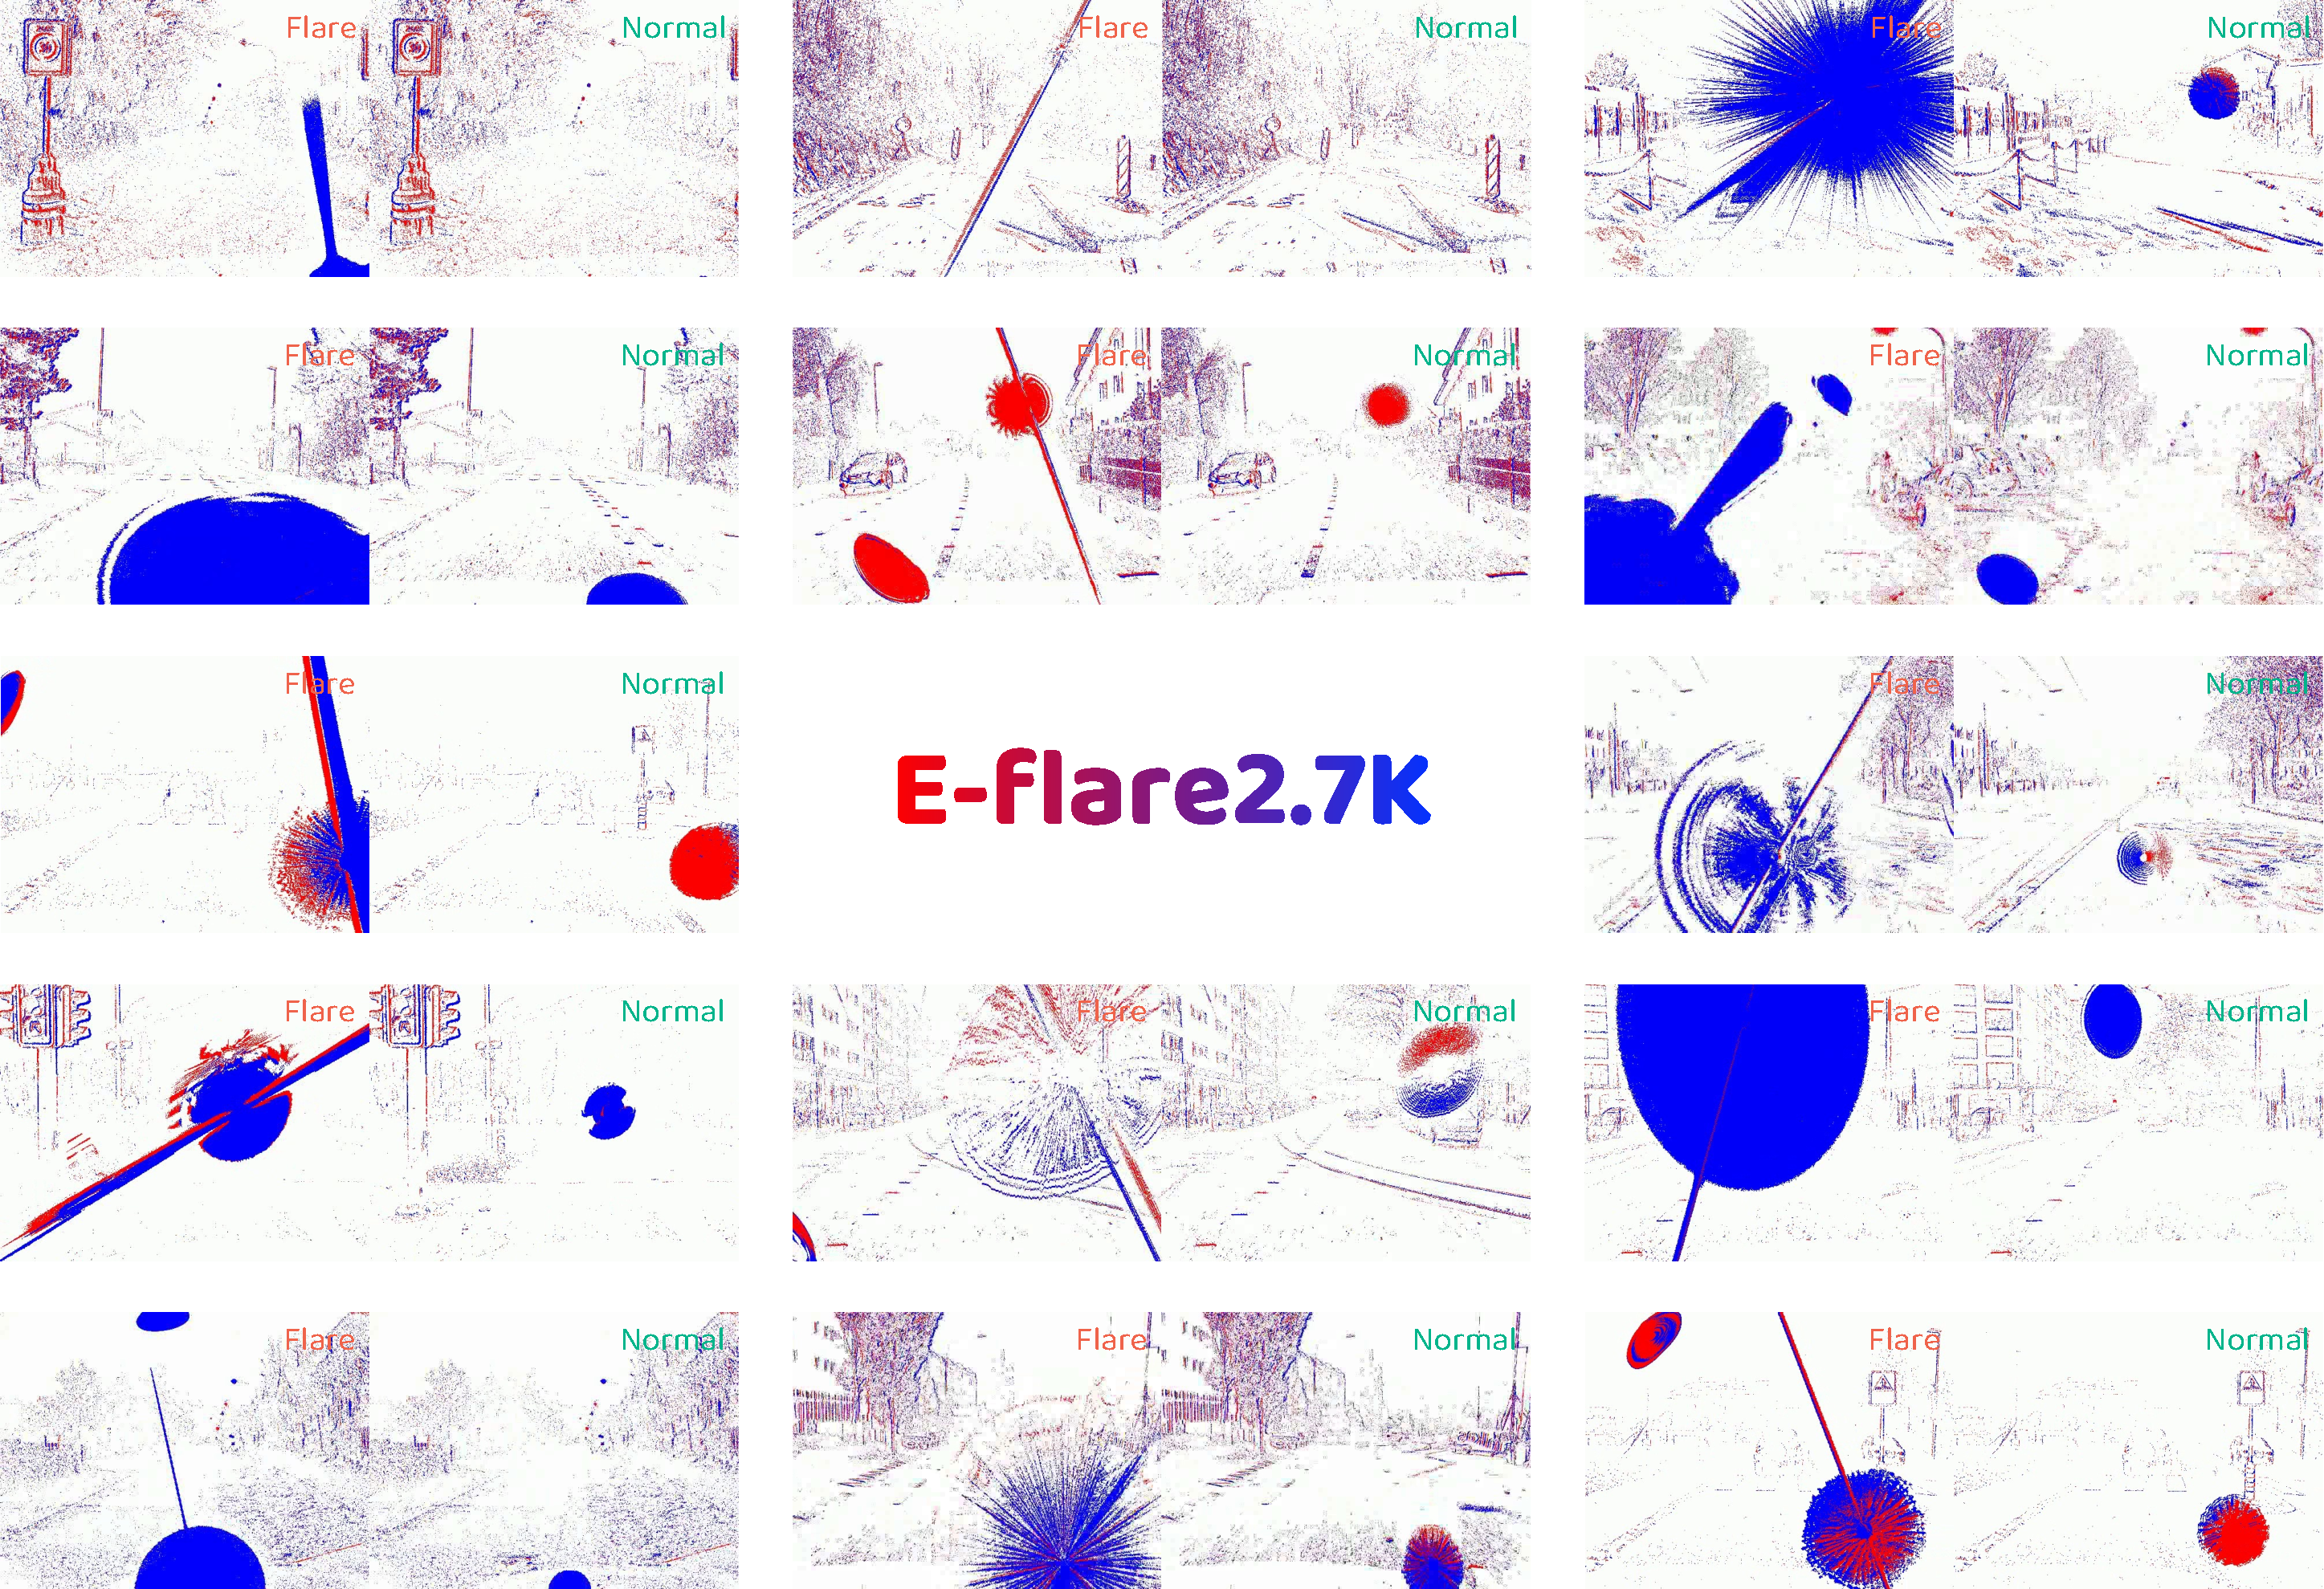
\includegraphics[width=\textwidth]{figures_supp/dataset_e-flare.pdf}
    \caption{\textbf{Examples from E-Flare2.7K.} This large-scale paired dataset combines synthetic event data under \textbf{\textcolor{ev_red}{flare}} (left) and \textbf{\textcolor{ev_green}{normal}} (right) conditions. Best viewed in color and zoomed in for details.}
    \label{APfig:dataset_eflare}
\end{figure}


\subsection{E-Flare-R: Real-World Paired Dataset}
\label{app:eflare_r_details}

\textbf{E-Flare-R} is the first paired real-world benchmark for event-based de-flaring, capturing the same scene under distinct optical impulse responses.

\noindent\textbf{Acquisition Setup.}
A Prophesee EVK4-HD event camera ($1280 \times 720$) is used with a custom rig of removable optical filters (six-point star filter and random-pattern filters). High-intensity light sources, including a frequency-controllable point light and a square Tungsten lamp, are placed within the FoV to produce diverse flare artifacts.

\noindent\textbf{Capture Protocol.}
A strict two-pass protocol is executed per scene: (1) \textbf{Observation Pass}: scene recorded with filter mounted; (2) \textbf{Reference Pass}: filter immediately removed, same scene re-recorded with camera rigidly static.

\noindent\textbf{Post-Processing.}
Raw recordings undergo metric-guided temporal alignment (cross-correlation of polarity signatures), reference cleaning via light-source geometry masks, noise injection to prevent overfitting, and center-cropping to $640 \times 480$ in $100$~ms windows. This yields $30$ high-quality paired sequences, each further divided into five $20$~ms segments during evaluation, for a total of $150$ paired samples. Representative samples are shown in Fig.~\ref{APfig:dataset_eflarer}.

\begin{figure}[H]
    \centering
    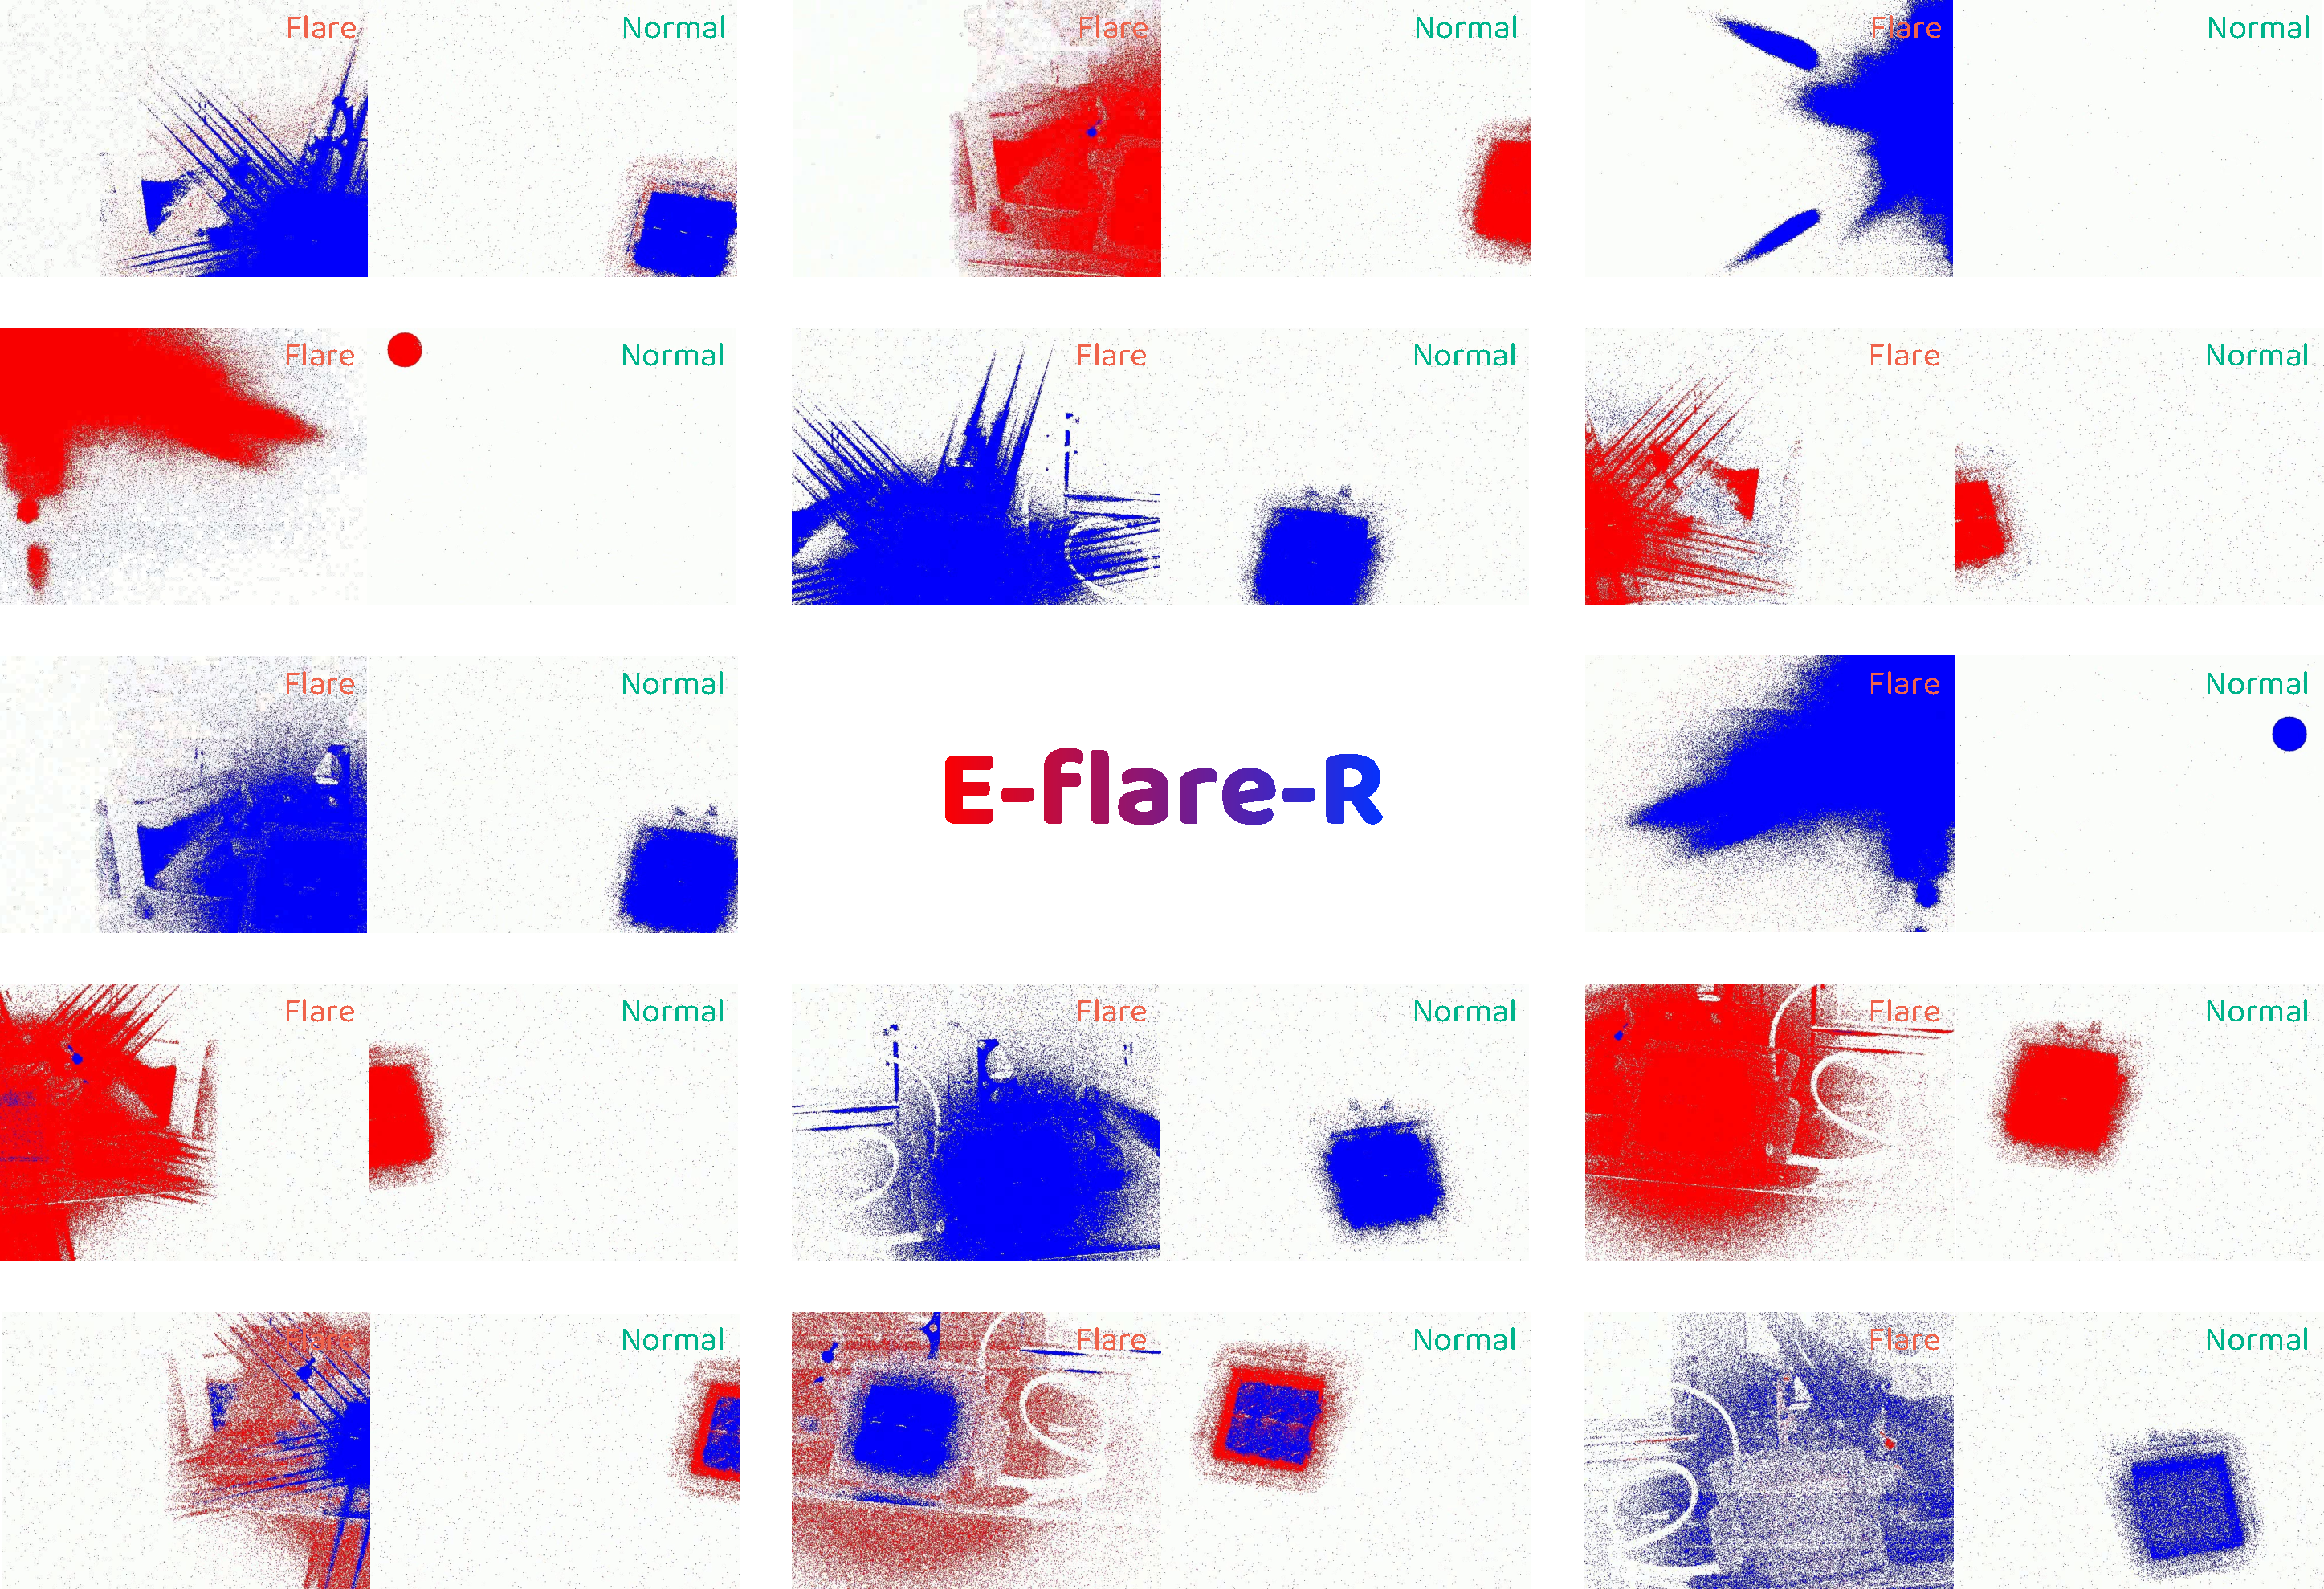
\includegraphics[width=\textwidth]{figures_supp/dataset_e-flare-r.pdf}
    \caption{\textbf{Examples from E-Flare-R.} This real-world paired dataset combines acquired event data under \textbf{\textcolor{ev_red}{flare}} (left) and \textbf{\textcolor{ev_green}{normal}} (right) conditions. Best viewed in color and zoomed in for details.}
    \label{APfig:dataset_eflarer}
\end{figure}


\subsection{DSEC-Flare: Curated Real-World Examples}
\label{app:dsec_flare_details}

\textbf{DSEC-Flare} comprises challenging sequences from the left camera ($640 \times 480$) of DSEC~\cite{gehrig2021dsec}, categorized into two groups:
\begin{itemize}
    \item \textbf{Periodic Streetlight Flare:} Sequences \texttt{zurich\_city\_03\_a}, \texttt{zurich\_city\_10\_b}, and \texttt{zurich\_city\_12\_a}, dominated by high-intensity streetlights producing strong periodic flare bursts as the camera passes underneath.
    \item \textbf{Complex Urban Flare:} Sequences \texttt{zurich\_city\_09\_c} and \texttt{zurich\_city\_09\_d}, featuring overlapping artifacts from vehicle headlights, traffic signals, and storefront illumination, testing generalization to diverse mixed-source flare.
\end{itemize}
As no paired ground truth is available, DSEC-Flare is used exclusively for qualitative evaluation. Representative examples are shown in Fig.~\ref{APfig:dataset_dsec}.

\begin{figure}[H]
    \centering
    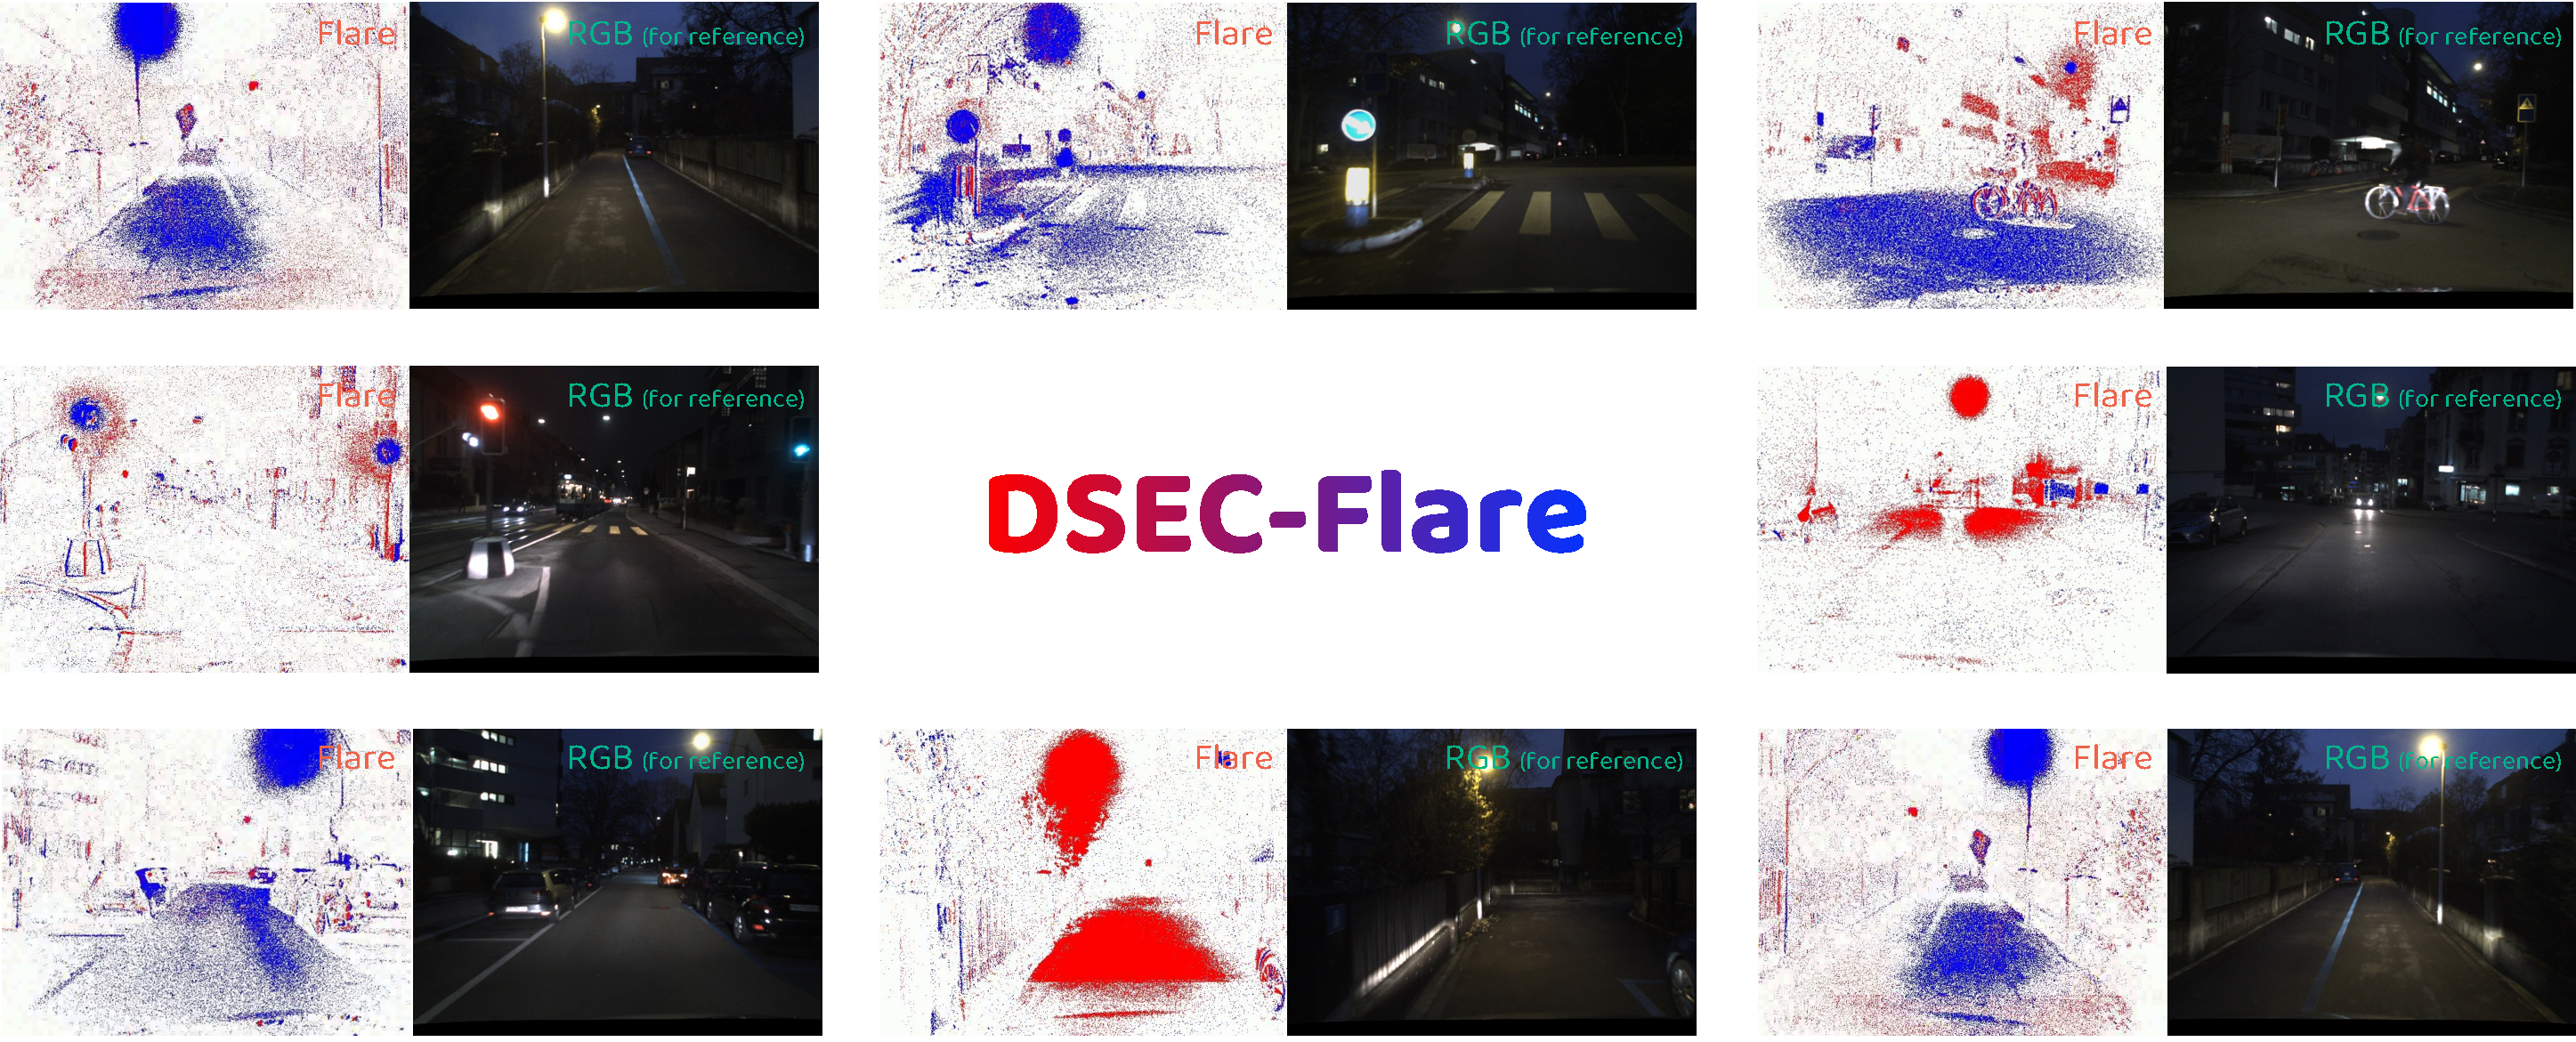
\includegraphics[width=\textwidth]{figures_supp/dataset_dsec-flare.pdf}
    \caption{\textbf{Examples from DSEC-Flare.} Real-world lens flare from vehicle lights and street lamps in driving scenarios. Each example shows the raw event stream alongside a reference RGB frame illustrating the light sources causing the artifacts. Best viewed in color and zoomed in for details.}
    \label{APfig:dataset_dsec}
\end{figure}


%% ============================================================
%% §B  Detailed Derivation of the Forward Model
%%     （保留 ECCV 更新版本：使用 ξ(t)/Φ(τ) 新符号，无 E_ideal）
%% ============================================================

\section{Detailed Derivation of the Forward Model}
\label{APapp:derivation}

The complete methodology pipeline is illustrated in Fig.~2 of the main paper.
This section expands on the theoretical forward model underpinning that pipeline.

\subsection{The Physical Origin of Lens Flare}
\label{APssec:flare_physics_and_data_impasse}

To understand why event cameras are susceptible to lens flare, we first formalize the universal imaging process. Any camera's output is the result of a two-stage pipeline: a lens system $\mathcal{L}$ that forms an irradiance map on the sensor plane, followed by a sensor $\mathcal{S}$ that converts this irradiance into a digital signal. An ideal lens, $\mathcal{L}_{\mathrm{ideal}}$, would perfectly map scene radiance to a clean sensor irradiance. However, a real lens, $\mathcal{L}_{\mathrm{real}}$, introduces aberrations. Lens flare is this corruption. It comprises two primary, highly complex components. \textbf{Scattering flare} arises from imperfections like dust or scratches, creating diffuse haze and radial streaks. \textbf{Reflection flare} is caused by unintended reflections between lens surfaces (a lens with $n$ elements has $n(2n-1)$ potential reflection paths), forming highly structured but diverse patterns like blobs and rings. Fortunately, as flare is a high-intensity phenomenon, it can be effectively approximated by a linear superposition in the intensity domain~\cite{dai2022flare7k,wu2021train,dai2024flare7k++}:
%
\begin{equation}
    \mathbf{I}_{\mathrm{ob}}(x, y, t) \approx \mathbf{I}_{\mathrm{bg}}(x, y, t) + \mathbf{I}_{\textcolor{ev_red}{\mathrm{\mathbf{f}}}}(x, y, t),
    \label{APeq:image_superposition}
\end{equation}
%
where $\mathbf{I}_{\mathrm{bg}}$ is the background irradiance and $\mathbf{I}_{\textcolor{ev_red}{\mathrm{\mathbf{f}}}}$ is the flare component, subsuming both the corrupted light source and the scattered flare energy. This corresponds to Eq.~\ref*{eq:image_superposition_final} of the main paper.

The critical insight is that this corruption happens in the lens, \textit{before} the sensor. The distinction between camera types lies in their sensor operator $\mathcal{S}$. For a conventional camera, the sensor integrates the already-corrupted irradiance over an exposure time $T$:
%
\begin{equation}
    V = \mathcal{S}_{\mathrm{RGB}}(\mathbf{I}_{\mathrm{ob}}(t)) = \int_{0}^{T} \mathbf{I}_{\mathrm{ob}}(\tau) \, d\tau~.
\end{equation}
%
\textbf{Overexposure} occurs when the integrated value exceeds the sensor's dynamic range, a fundamental limitation of $\mathcal{S}_{\mathrm{RGB}}$.

An event camera's sensor, $\mathcal{S}_{\mathrm{evt}}(\cdot)$, operates on a different principle. As established in Eq.~\ref*{eq:event_stream_definition} of the main paper, the resulting event stream is a sum of signed impulses:
%
\begin{equation}
    \mathbf{E}(t) = \mathcal{S}_{\mathrm{evt}}(\mathbf{I}_{\mathrm{ob}}(t)) = \sum\nolimits_{i} p_i \delta(t - t_i)~,
\end{equation}
%
where $\delta(\cdot)$ is the Dirac delta and $p_i \in \{+1,-1\}$ is the polarity. Since the flare irradiance $\mathbf{I}_{\textcolor{ev_red}{\mathrm{\mathbf{f}}}}(t)$ is itself a time-varying signal, it introduces intensity changes that the event sensor faithfully reports as spurious events, corrupting the true scene dynamics. An event camera therefore does \emph{not} confer immunity to lens flare: the artifact is embedded in the light signal before any sensor is involved.

This establishes the event de-flaring task as an inverse problem: recovering the clean event stream from the contaminated observation $\mathbf{E}_{\mathrm{ob}}$. The complexity precludes simple filter-based solutions, as lens flare fundamentally alters the entire spatio-temporal distribution of events, making it impossible to classify individual events as ``signal'' or ``artifact'' in isolation. A learning-based approach is therefore the most viable path, but it requires paired training data, which in turn requires a quantitative understanding of the forward process.


\subsection{Step-by-Step Derivation of the Forward Model}
\label{APssec:event_synthesis_model}

We now expand on Eqs.~\ref*{eq:sensor_model_integral_redef}--\ref*{eq:integrand_phi} of the main paper, providing the full derivation chain.

\paragraph{Step 1: Dual Representation of the Event Stream.}

Although the event stream $\mathbf{E}(t)$ is discrete, it admits a continuous interpretation through its relationship to the log-intensity $L(t) = \log(\mathbf{I}_{\mathrm{ob}}(t))$. Because each pixel accumulates event impulses until the total log-change reaches the threshold $c$, the following integral identity holds (Eq.~\ref*{eq:sensor_model_integral_redef} of the main paper):
%
\begin{equation}
    L(t) = c \int_{0}^{t} \mathbf{E}(\tau) \, d\tau + L(0) + \varepsilon(t)~,
    \label{APeq:sensor_integral}
\end{equation}
%
where $L(0)$ is the initial log-intensity and $\varepsilon(t)$ is the \emph{total intensity residual}. This term aggregates \emph{all} signal components not encoded in the event stream. It comprises two parts: (1) the \textbf{sub-threshold quantization error}, bounded in magnitude by $c$, and (2) \textbf{sensor noise} (\eg, shot noise, threshold variance), which is stochastic and may accumulate over time. While modern sensors minimize noise, $\varepsilon(t)$ remains an intrinsic part of the physical process.

Taking the time derivative of Eq.~\ref{APeq:sensor_integral} yields the \emph{continuous link} (Eq.~\ref*{eq:continuous_link} of the main paper):
%
\begin{equation}
    \frac{dL(t)}{dt} = c \cdot \mathbf{E}(t) + \xi(t)~, \quad \xi(t) \triangleq \frac{d\varepsilon(t)}{dt}~.
    \label{APeq:continuous_link}
\end{equation}
%
This decomposes the log-intensity rate into an impulsive term ($c \cdot \mathbf{E}$, encoding discrete events) and a residual rate ($\xi$, encoding sub-threshold drift and noise). Importantly, this equation holds as an \emph{identity}: $\xi(t)$ is \emph{defined} to absorb whatever remains after subtracting $c \cdot \mathbf{E}(t)$, so no approximation is involved.

\paragraph{Step 2: Log-Derivative Mixing.}

We now translate the intensity superposition (Eq.~\ref{APeq:image_superposition}) into the log domain. Let $L_{\mathrm{ob}} = \log(\mathbf{I}_{\mathrm{bg}} + \mathbf{I}_{\textcolor{ev_red}{\mathrm{\mathbf{f}}}})$. Taking the time derivative via the chain rule and separating the contributions (all quantities are functions of $t$; we suppress the argument in the intermediate fractions for readability):
%
\begin{align}
    \frac{dL_{\mathrm{ob}}(t)}{dt}
    &= \frac{\dot{\mathbf{I}}_{\mathrm{bg}} + \dot{\mathbf{I}}_{\textcolor{ev_red}{\mathrm{\mathbf{f}}}}}{\mathbf{I}_{\mathrm{bg}} + \mathbf{I}_{\textcolor{ev_red}{\mathrm{\mathbf{f}}}}} \notag \\
    &= \frac{\mathbf{I}_{\mathrm{bg}}}{\mathbf{I}_{\mathrm{bg}} + \mathbf{I}_{\textcolor{ev_red}{\mathrm{\mathbf{f}}}}} \cdot \frac{\dot{\mathbf{I}}_{\mathrm{bg}}}{\mathbf{I}_{\mathrm{bg}}}
     + \frac{\mathbf{I}_{\textcolor{ev_red}{\mathrm{\mathbf{f}}}}}{\mathbf{I}_{\mathrm{bg}} + \mathbf{I}_{\textcolor{ev_red}{\mathrm{\mathbf{f}}}}} \cdot \frac{\dot{\mathbf{I}}_{\textcolor{ev_red}{\mathrm{\mathbf{f}}}}}{\mathbf{I}_{\textcolor{ev_red}{\mathrm{\mathbf{f}}}}} \notag \\
    &= w_{\mathrm{bg}}(t)\,\frac{dL_{\mathrm{bg}}(t)}{dt} + w_{\textcolor{ev_red}{\mathrm{\mathbf{f}}}}(t)\,\frac{dL_{\textcolor{ev_red}{\mathrm{\mathbf{f}}}}(t)}{dt}~,
    \label{APeq:log_deriv_mixing}
\end{align}
%
where $\dot{\mathbf{I}} \triangleq d\mathbf{I}/dt$ and the intensity-weighted coefficients are defined as:
%
\begin{equation}
    w_{\mathrm{bg}}(t) = \frac{\mathbf{I}_{\mathrm{bg}}(t)}{\mathbf{I}_{\mathrm{bg}}(t) + \mathbf{I}_{\textcolor{ev_red}{\mathrm{\mathbf{f}}}}(t)}~, \quad w_{\textcolor{ev_red}{\mathrm{\mathbf{f}}}}(t) = 1 - w_{\mathrm{bg}}(t)~.
    \label{APeq:weights}
\end{equation}
%
Although intensities superpose \emph{linearly}, their log-derivatives mix through a \emph{weighted sum} governed by the relative intensity ratio. This is the mathematical origin of the \textbf{non-linear suppression effect}: when flare dominates ($\mathbf{I}_{\textcolor{ev_red}{\mathrm{\mathbf{f}}}} \gg \mathbf{I}_{\mathrm{bg}}$), $w_{\mathrm{bg}} \to 0$, and background log-changes are suppressed in the observed signal.

\paragraph{Step 3: Substituting the Dual Representation.}

We apply the continuous link (Eq.~\ref{APeq:continuous_link}) separately to each component ($\mathrm{bg}$ and $\textcolor{ev_red}{\mathrm{\mathbf{f}}}$) and substitute into Eq.~\ref{APeq:log_deriv_mixing}:
%
\begin{equation}
    \frac{dL_{\mathrm{ob}}(t)}{dt} = w_{\mathrm{bg}}(t) \!\left[ c\,\mathbf{E}_{\mathrm{bg}}(t) + \xi_{\mathrm{bg}}(t) \right]
    + w_{\textcolor{ev_red}{\mathrm{\mathbf{f}}}}(t) \!\left[ c\,\mathbf{E}_{\textcolor{ev_red}{\mathrm{\mathbf{f}}}}(t) + \xi_{\textcolor{ev_red}{\mathrm{\mathbf{f}}}}(t) \right]~,
    \label{APeq:full_mixing_deriv}
\end{equation}
%
where $\xi_{\mathrm{bg}}(t)$ and $\xi_{\textcolor{ev_red}{\mathrm{\mathbf{f}}}}(t)$ denote the respective residual rates of each component. This is the expanded form of Eq.~\ref*{eq:full_mixing_derivative} in the main paper.

\paragraph{Step 4: The Complete Forward Model.}

Integrating Eq.~\ref{APeq:full_mixing_deriv} from $0$ to $t$ gives $L_{\mathrm{ob}}(t) = \int_0^t \Phi(\tau)\,d\tau + L_{\mathrm{ob}}(0)$, where we define the \emph{mixed log-rate potential}:
%
\begin{equation}
    \Phi(\tau) =
    \underbrace{w_{\mathrm{bg}}(\tau)\, c\,\mathbf{E}_{\mathrm{bg}}(\tau) + w_{\textcolor{ev_red}{\mathrm{\mathbf{f}}}}(\tau)\, c\,\mathbf{E}_{\textcolor{ev_red}{\mathrm{\mathbf{f}}}}(\tau)}_{\text{Weighted Impulse Interaction}}
    + \underbrace{w_{\mathrm{bg}}(\tau)\,\xi_{\mathrm{bg}}(\tau) + w_{\textcolor{ev_red}{\mathrm{\mathbf{f}}}}(\tau)\,\xi_{\textcolor{ev_red}{\mathrm{\mathbf{f}}}}(\tau)}_{\xi_{\mathrm{mix}}}~.
    \label{APeq:phi_definition}
\end{equation}
%
Reconstructing the observed irradiance as $\mathbf{I}_{\mathrm{ob}}(t) = \exp(L_{\mathrm{ob}}(t))$ and applying the sensor operator yields the complete forward model:
%
\begin{equation}
    \mathbf{E}_{\mathrm{ob}}(t) = \mathcal{S}_{\mathrm{evt}}\!\left( \exp\!\left( \int_{0}^{t} \Phi(\tau)\,d\tau + L_{\mathrm{ob}}(0) \right) \right)~.
    \label{APeq:forward_model}
\end{equation}
%
This matches Eqs.~\ref*{eq:full_forward_model}--\ref*{eq:integrand_phi} of the main paper. The outer $\mathcal{S}_{\mathrm{evt}}$ ensures the output is a physically valid discrete event stream; the integral captures the accumulated log-intensity change, explaining why flare-dominated regions exhibit slower accumulation and thus suppressed background events. The term $\xi_{\mathrm{mix}}$ aggregates the residual contributions from both components.

\paragraph{Step 5: Why Direct Simulation is Intractable.}

Directly evaluating Eq.~\ref{APeq:forward_model} requires (i) the continuous per-pixel intensity profiles $\mathbf{I}_{\mathrm{bg}}(t)$ and $\mathbf{I}_{\textcolor{ev_red}{\mathrm{\mathbf{f}}}}(t)$ at every instant to compute the weights $w(t)$, and (ii) access to $\xi_{\mathrm{mix}}$ to model residual effects. In practice, we observe only two discrete event streams without continuous intensity access. This intractability motivates the PNL-ES approximation described in Sec.~\ref*{ssec:simulator} and expanded in the following section.


\subsection{From the Forward Model to PNL-ES}
\label{APssec:simulator_implementation}

With the complete forward model established (Eq.~\ref{APeq:forward_model}), we now describe how our Physics-guided Non-Linear Event Suppression (PNL-ES) operator implements it in practice.

\paragraph{The Simplified Principle.}

In high-dynamic-range event camera regimes, signal energy concentrates in the impulse terms ($c\cdot\mathbf{E}$); the mixed residual $\xi_{\mathrm{mix}}$ is small relative to the weighted impulse terms. Setting $\xi_{\mathrm{mix}} \approx 0$, the potential simplifies to:
%
\begin{equation}
    \Phi(\tau) \approx c\left[ w_{\mathrm{bg}}(\tau)\,\mathbf{E}_{\mathrm{bg}}(\tau) + w_{\textcolor{ev_red}{\mathrm{\mathbf{f}}}}(\tau)\,\mathbf{E}_{\textcolor{ev_red}{\mathrm{\mathbf{f}}}}(\tau) \right]~.
\end{equation}
%
This reveals the core physical principle: the instantaneous event rate of the mixture is an intensity-weighted combination of the source event rates. PNL-ES implements this by treating $w_{\mathrm{bg}}(t)$ as the \emph{retention probability} for each background event, and $w_{\textcolor{ev_red}{\mathrm{\mathbf{f}}}}(t)$ for each flare event. The complete procedure is given in Algorithm~\ref{APalg:event_mixing}. Our goal is distribution matching over real-world data, not exact single-instance replication; the remaining $\xi_{\mathrm{mix}}$ contribution is handled through probabilistic sampling and noise augmentation during training.


\begin{algorithm}[t]
\caption{Physics-Grounded Event Stream Mixing (PNL-ES)}
\label{APalg:event_mixing}
\begin{algorithmic}[1]
\Statex \textbf{Input:} Events $E_a$, $E_b$; Intensities $I_a(t)$, $I_b(t)$
\Statex \textbf{Output:} Mixed events: $\text{Mix}(E_a, E_b)$
\Statex
\State $E_{\text{mixed}} \leftarrow \emptyset$
\State Compute weights: $w_a(t) = I_a(t)/(I_a(t)+I_b(t))$, \; $w_b(t) = 1-w_a(t)$
\For{each event $e_i$ in $E_a$}
    \If{$\text{random}() < w_a(e_i.t)$}
        \State Add $e_i$ to $E_{\text{mixed}}$
    \EndIf
\EndFor
\For{each event $e_j$ in $E_b$}
    \If{$\text{random}() < w_b(e_j.t)$}
        \State Add $e_j$ to $E_{\text{mixed}}$
    \EndIf
\EndFor
\State \Return $E_{\text{mixed}}$ sorted by timestamps
\end{algorithmic}
\end{algorithm}


\paragraph{Constructing Training Pairs.}

To generate supervised training data, we decompose the scene into three components:
\begin{itemize}
\item \textbf{$\mathbf{E}_{\mathrm{bg}}$}: background events, free of the primary light source.
\item \textbf{$\mathbf{E}_{\textcolor{ev_red}{\mathrm{\mathbf{f}}}}$}: events from the light source under a non-ideal lens (with flare).
\item \textbf{$\mathbf{E}_{\mathrm{light}}$}: events from the light source under an ideal lens (clean reference).
\end{itemize}
Applying the Mix operator (Algorithm~\ref{APalg:event_mixing}) yields the paired training samples:
%
\begin{align}
\mathbf{E}_{\mathrm{ob}} &= \mathrm{Mix}(\mathbf{E}_{\mathrm{bg}},\, \mathbf{E}_{\textcolor{ev_red}{\mathrm{\mathbf{f}}}}) \label{APeq:compose_obs} \\
\mathbf{E}_{\mathrm{gt}} &= \mathrm{Mix}(\mathbf{E}_{\mathrm{bg}},\, \mathbf{E}_{\mathrm{light}}) \label{APeq:compose_gt}
\end{align}
%
Generating the required data assets follows the pipeline described in Sec.~\ref*{ssec:simulator} of the main paper. The intensity profiles $\mathbf{I}_{\textcolor{ev_red}{\mathrm{\mathbf{f}}}}(t)$ and $\mathbf{I}_{\mathrm{light}}(t)$ for computing retention probabilities are derived from synthetic videos generated from Flare7K++~\cite{dai2024flare7k++} assets; the background profile $\mathbf{I}_{\mathrm{bg}}(t)$ is estimated from the available event data ($\mathbf{E}_{\mathrm{bg}}$) via standard intensity reconstruction from DSEC~\cite{gehrig2021dsec} sequences, providing a relative intensity proxy sufficient for the probabilistic PNL-ES formulation.

\paragraph{Learning to Deflare.}
With paired data $(\mathbf{E}_{\mathrm{ob}}, \mathbf{E}_{\mathrm{gt}})$, we frame de-flaring as a supervised learning task. Events are encoded into spatio-temporal voxel grids $\mathcal{V}_{\mathrm{ob}}$ and $\mathcal{V}_{\mathrm{gt}}$. We employ a 3D U-Net~\cite{cciccek20163d} in a residual learning formulation:
%
\begin{equation}
\mathcal{V}_{\mathrm{pred}} = \mathcal{V}_{\mathrm{ob}} + \text{U-Net}(\mathcal{V}_{\mathrm{ob}})~,
\end{equation}
%
trained by minimizing MSE between $\mathcal{V}_{\mathrm{pred}}$ and $\mathcal{V}_{\mathrm{gt}}$. Further implementation details are provided in the sections below.


%% ============================================================
%% §C  E-DeflareNet: Network and Codec Details
%% ============================================================

\section{Implementation Details of the Network and Codec}
\label{app:network_details}

This section provides further details on the implementation of our de-flaring network and the event-to-voxel codec.

\subsection{Network Architecture Details}
\textbf{E-DeflareNet} employs a standard residual \textbf{TrueResidualUNet3D} architecture following the residual learning principle: $\hat{\mathcal{V}}_{\mathrm{gt}} = \mathcal{V}(\mathbf{E}_{\mathrm{ob}}) + f_{\theta}(\mathcal{V}(\mathbf{E}_{\mathrm{ob}}))$. The backbone $f_{\theta}$ is adapted from \textbf{ResidualUNet3D} in the \textit{pytorch-3dunet} library. A critical design choice is the zero-initialization of the final $1\times1\times1$ convolution, ensuring $f_{\theta}(\cdot) \approx 0$ at initialization. This forces an initial identity mapping, allowing the model to focus on learning the negative flare residual.

As illustrated in Fig.~\ref{APfig:architecture}, the network is a 4-level U-Net with $\sim$$7.07$M parameters. It accepts single-channel voxel grids of shape $(B, 1, 8, 480, 640)$. The encoder utilizes residual blocks and 3D max-pooling to downsample features, while the symmetric decoder uses transposed convolutions for upsampling. Skip connections concatenate encoder features with the decoder path, integrating multi-scale context for high-fidelity restoration.

\begin{figure}[H]
    \centering
    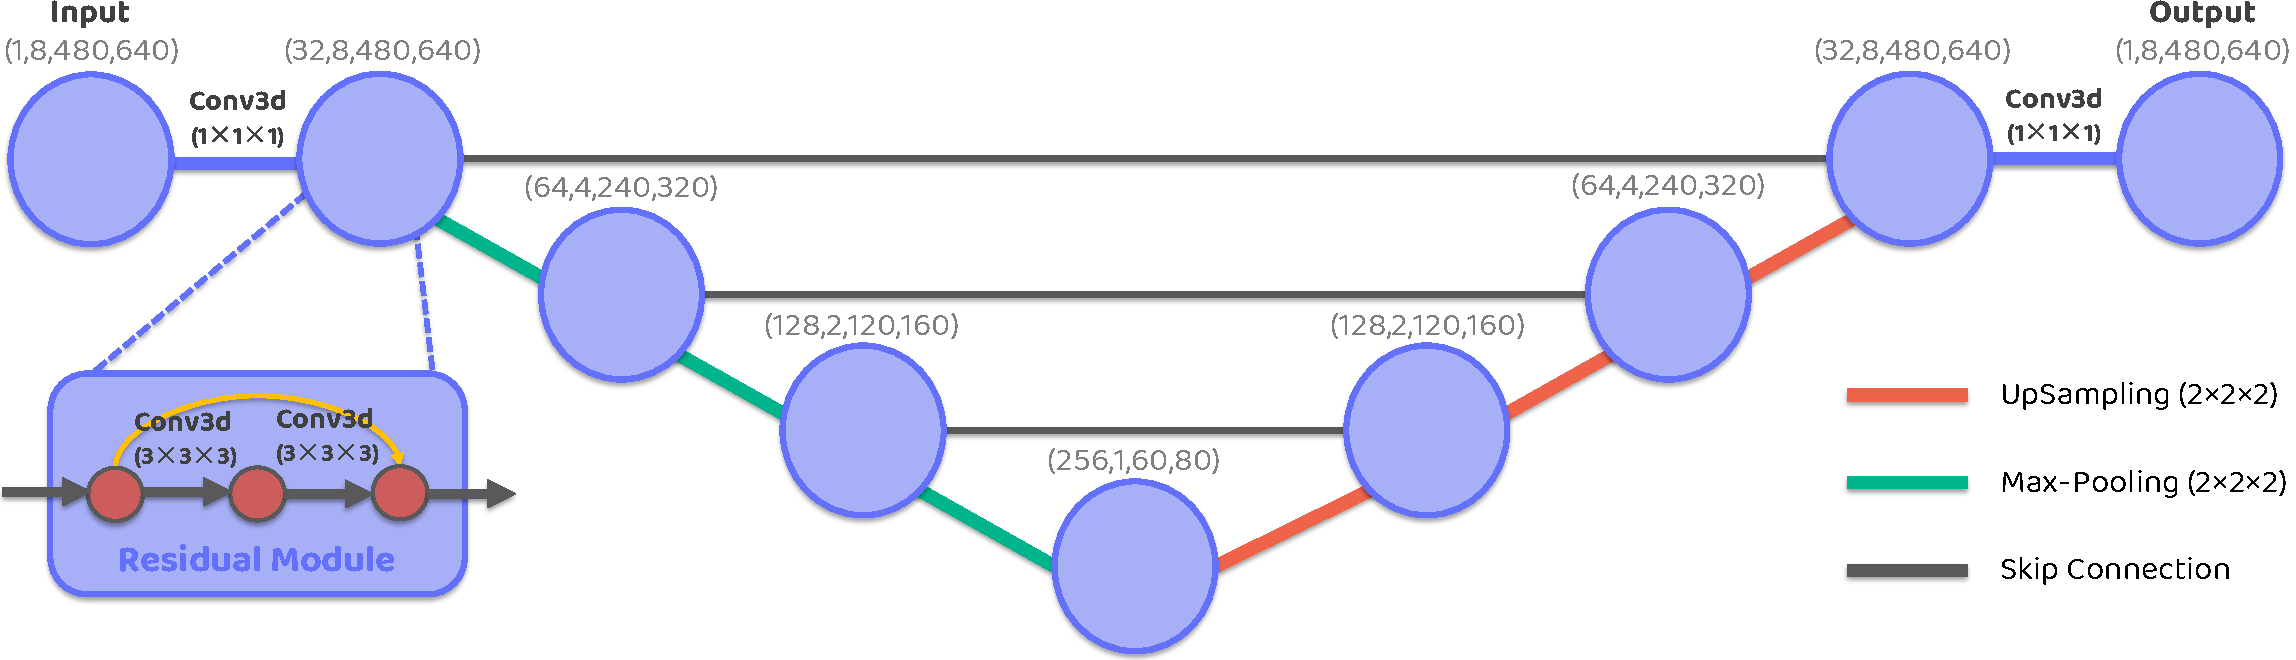
\includegraphics[width=\textwidth, clip=true]{figures_supp/architecture_v2.pdf}
    \caption{\textbf{E-DeflareNet Architecture.} The network is a standard $4$-level Residual 3D U-Net, featuring a symmetric encoder--decoder structure with skip connections to combine multi-scale features for high-fidelity event-based restoration.}
    \label{APfig:architecture}
\end{figure}

\subsection{Training Details}
\label{app:training_details}
E-DeflareNet is implemented in PyTorch and optimized with the \textbf{Adam} optimizer (initial learning rate $2 \times 10^{-4}$, weight decay $1 \times 10^{-5}$). The learning rate is annealed via a \texttt{MultiStepLR} scheduler, decaying by a factor of $0.2$ at epochs $10$, $20$, and $30$. Training uses a batch size of $2$ on a single NVIDIA RTX~3090 GPU, with the final model selected at iteration $40{,}000$. To ensure training stability, the output layer uses an identity activation (no sigmoid/softmax), and the zero-initialized final convolution guarantees a perfect identity mapping at initialization.

\subsection{Event-to-Voxel Encoding Algorithm}
The encoding operator $\mathcal{V}(\cdot)$ transforms an event stream $\mathbf{E} = \{e_k\}_{k=1}^N$ over a duration $T$ ($20$~ms) into a voxel grid $\mathcal{V} \in \mathbb{R}^{B_\mathrm{bins} \times H \times W}$. Each event is a tuple $e_k = (t_k, x_k, y_k, p_k)$. The process proceeds as follows:
\begin{enumerate}
    \item \textbf{Initialization:} A zero tensor $\mathcal{V}$ of size $(B_\mathrm{bins}, H, W)$ is created, where $B_\mathrm{bins}=8$ is the number of temporal bins.
    \item \textbf{Temporal Binning:} The duration $T$ is divided into $B_\mathrm{bins}$ uniform intervals of duration $\Delta t = T/B_\mathrm{bins}$. For each event $e_k$, its bin index $b_k = \lfloor (t_k - t_0) / \Delta t \rfloor$, where $t_0$ is the first event timestamp.
    \item \textbf{Polarity Accumulation:} The polarity of each event is accumulated at its spatio-temporal cell:
    \begin{equation}
        \mathcal{V}(b, y, x) = \sum\nolimits_{k:\,(x_k, y_k, b_k) = (x, y, b)} p_k~.
    \end{equation}
\end{enumerate}
This process is implemented via efficient vectorized PyTorch operations.

\subsection{Voxel-to-Event Decoding Algorithm}
The decoding operator $\mathcal{V}^{-1}(\cdot)$ converts a restored voxel grid $\hat{\mathcal{V}}_{\mathrm{gt}}$ back into an event stream $\hat{\mathbf{E}}_{\mathrm{gt}}$:
\begin{enumerate}
    \item \textbf{Event Count Determination:} For each cell $(b, y, x)$, its floating-point value is rounded to the nearest integer $n = \mathrm{round}(\hat{\mathcal{V}}_{\mathrm{gt}}(b, y, x))$. The magnitude $|n|$ determines the number of events; $\mathrm{sgn}(n)$ determines their polarity.
    \item \textbf{Timestamp Generation:} For the $|n|$ events from bin $b$, each is assigned a random timestamp $t \sim \mathcal{U}(b \cdot \Delta t,\, (b{+}1) \cdot \Delta t)$, restoring the asynchronous nature of the event stream.
    \item \textbf{Stream Assembly \& Sorting:} All generated events are collected and sorted chronologically to produce the final valid event stream $\hat{\mathbf{E}}_{\mathrm{gt}}$.
\end{enumerate}


%% ============================================================
%% §D  Experimental Details
%% ============================================================

\section{Experimental Details}
\label{app:experimental_details}

This section provides comprehensive details regarding our experimental setup, including the implementation of baseline methods and the mathematical definitions of our evaluation metrics.

\subsection{Implementation Details of Baseline Methods}
\label{app:baselines_details}

    \subsubsection{EFR~\cite{wang2022linear}}
    Event Frequency Removal (EFR) is a linear comb filter targeting periodic noise. We configure it with a base frequency of $50$~Hz and the default primary feedback coefficient ($\rho_1 = 0.6$). The original implementation includes a $22$~ms warm-up phase that discards initial events; on our short test sequences this would cause unfair data loss. We therefore developed a Python wrapper that re-appends these warm-up events unmodified, ensuring evaluation over the complete temporal window.

    \subsubsection{PFD-A \& PFD-B~\cite{shi2024polarity}}
    We evaluate two variants of the polarity-flip denoising algorithm:
    \begin{itemize}
        \item \textbf{PFD-A} (\texttt{score\_select=1}): general-purpose event denoising using spatio-temporal correlation.
        \item \textbf{PFD-B} (\texttt{score\_select=0}): targeted at light-source artifacts via polarity-flipping patterns; a stronger and more relevant de-flaring baseline.
    \end{itemize}
    For both variants we use a temporal window of $20$~ms and a spatial neighborhood size of $3$, invoking the original C++ executable via a Python wrapper to ensure full algorithmic consistency.

    \subsubsection{Voxel Transform}
    The \emph{Voxel Transform} baseline serves as a control experiment isolating the contribution of E-DeflareNet from any implicit filtering effects of the codec. The input event stream is encoded into a voxel grid and immediately decoded back without any learned processing, effectively setting $f_{\theta}(\cdot) = 0$. Any performance improvement of our full model over this baseline is therefore directly attributable to the network's learned de-flaring capability.

\subsection{Detailed Definition of Evaluation Metrics}
\label{app:metrics_details}

    \subsubsection{Event-Level Metrics}
    These metrics treat event streams as 4D point clouds in $(t, x, y, p)$ space. Prior to computation, all four dimensions are normalized to $[0, 100]$ for balanced contribution.

    \noindent\textbf{Chamfer Distance (CD, $\downarrow$).}
    We use a one-sided variant that does not penalize correct removal of flare events:
    \begin{equation}
        \mathrm{CD}(\hat{\mathbf{E}}_{\mathrm{gt}}, \mathbf{E}_{\mathrm{gt}}) = \frac{1}{|\hat{\mathbf{E}}_{\mathrm{gt}}|} \sum_{e_i \in \hat{\mathbf{E}}_{\mathrm{gt}}} \min_{e_j \in \mathbf{E}_{\mathrm{gt}}} \| e_i - e_j \|_2~.
    \end{equation}

    \noindent\textbf{Gaussian Distance (GD, $\downarrow$).}
    A robust variant of CD that applies a Gaussian weighting to suppress outlier influence:
    \begin{equation}
        \mathrm{GD}(\hat{\mathbf{E}}_{\mathrm{gt}}, \mathbf{E}_{\mathrm{gt}}) = \frac{1}{|\hat{\mathbf{E}}_{\mathrm{gt}}|} \sum_{e_i \in \hat{\mathbf{E}}_{\mathrm{gt}}} \left(1 - \exp\!\left(-\frac{d_i^2}{\sigma}\right)\right)~,
    \end{equation}
    where $d_i^2 = \min_{e_j \in \mathbf{E}_{\mathrm{gt}}} \|e_i - e_j\|_2^2$ and $\sigma = 0.4$.

    \subsubsection{Voxel-Level Metrics}
    These metrics compare the restored voxel grid $\hat{\mathcal{V}}_{\mathrm{gt}}$ against the ground-truth grid $\mathcal{V}_{\mathrm{gt}} \in \mathbb{R}^{B_\mathrm{bins} \times H \times W}$ ($B_\mathrm{bins}=8$). All scores are averaged over $20$~ms segments.

    \noindent\textbf{MSE ($\downarrow$).} Strict voxel-wise squared error:
    \begin{equation}
        \mathrm{MSE}(\hat{\mathcal{V}}_{\mathrm{gt}}, \mathcal{V}_{\mathrm{gt}}) = \frac{1}{B_\mathrm{bins} \cdot H \cdot W} \sum_{b,y,x} \!\left( \hat{\mathcal{V}}_{\mathrm{gt}}(b,y,x) - \mathcal{V}_{\mathrm{gt}}(b,y,x) \right)^2\!.
    \end{equation}

    \noindent\textbf{PMSE ($\downarrow$).} Spatially tolerant variant via polarity separation and $k \times k$ average pooling before MSE; reported at $k=2$ and $k=4$.

    \noindent\textbf{F1-Score Variants ($\uparrow$).} Grids are binarized with threshold $\theta=0.001$ after polarity separation. Three variants with decreasing strictness:
    \begin{itemize}
        \item \textbf{R-F1}: computed on the full $2 \times B_\mathrm{bins} \times H \times W$ grid; requires precise space-time-polarity alignment.
        \item \textbf{T-F1}: temporal dimension collapsed by summation first; tolerant to small within-window timing shifts.
        \item \textbf{TP-F1}: both temporal and polarity dimensions collapsed; evaluates overall spatial event distribution only.
    \end{itemize}


%% ============================================================
%% §E  Additional Experimental Results
%% ============================================================

\section{Additional Experimental Results}
\label{app:more_results}

This section presents additional qualitative results to further demonstrate the effectiveness of our E-Deflare framework on a wider variety of challenging real-world and simulated scenes.

\subsection{Robustness in Typical Urban Scenarios}

Figs.~\ref{APfig:supp_1} and~\ref{APfig:supp_2} show scenarios typical of urban night driving, dominated by strong periodic interference from streetlights, a distribution closely mirroring real-world conditions in DSEC~\cite{gehrig2021dsec}. Aggressive filtering baselines suppress artifacts but erroneously remove valid background events, losing scene detail. General denoising methods (\eg, PFD-A) misinterpret large-scale structured flare as a valid signal, leaving artifacts intact. In contrast, \textbf{E-DeflareNet} accurately parses the flare structure, achieving precise removal while robustly preserving background event density.

\begin{figure}[H]
    \centering
    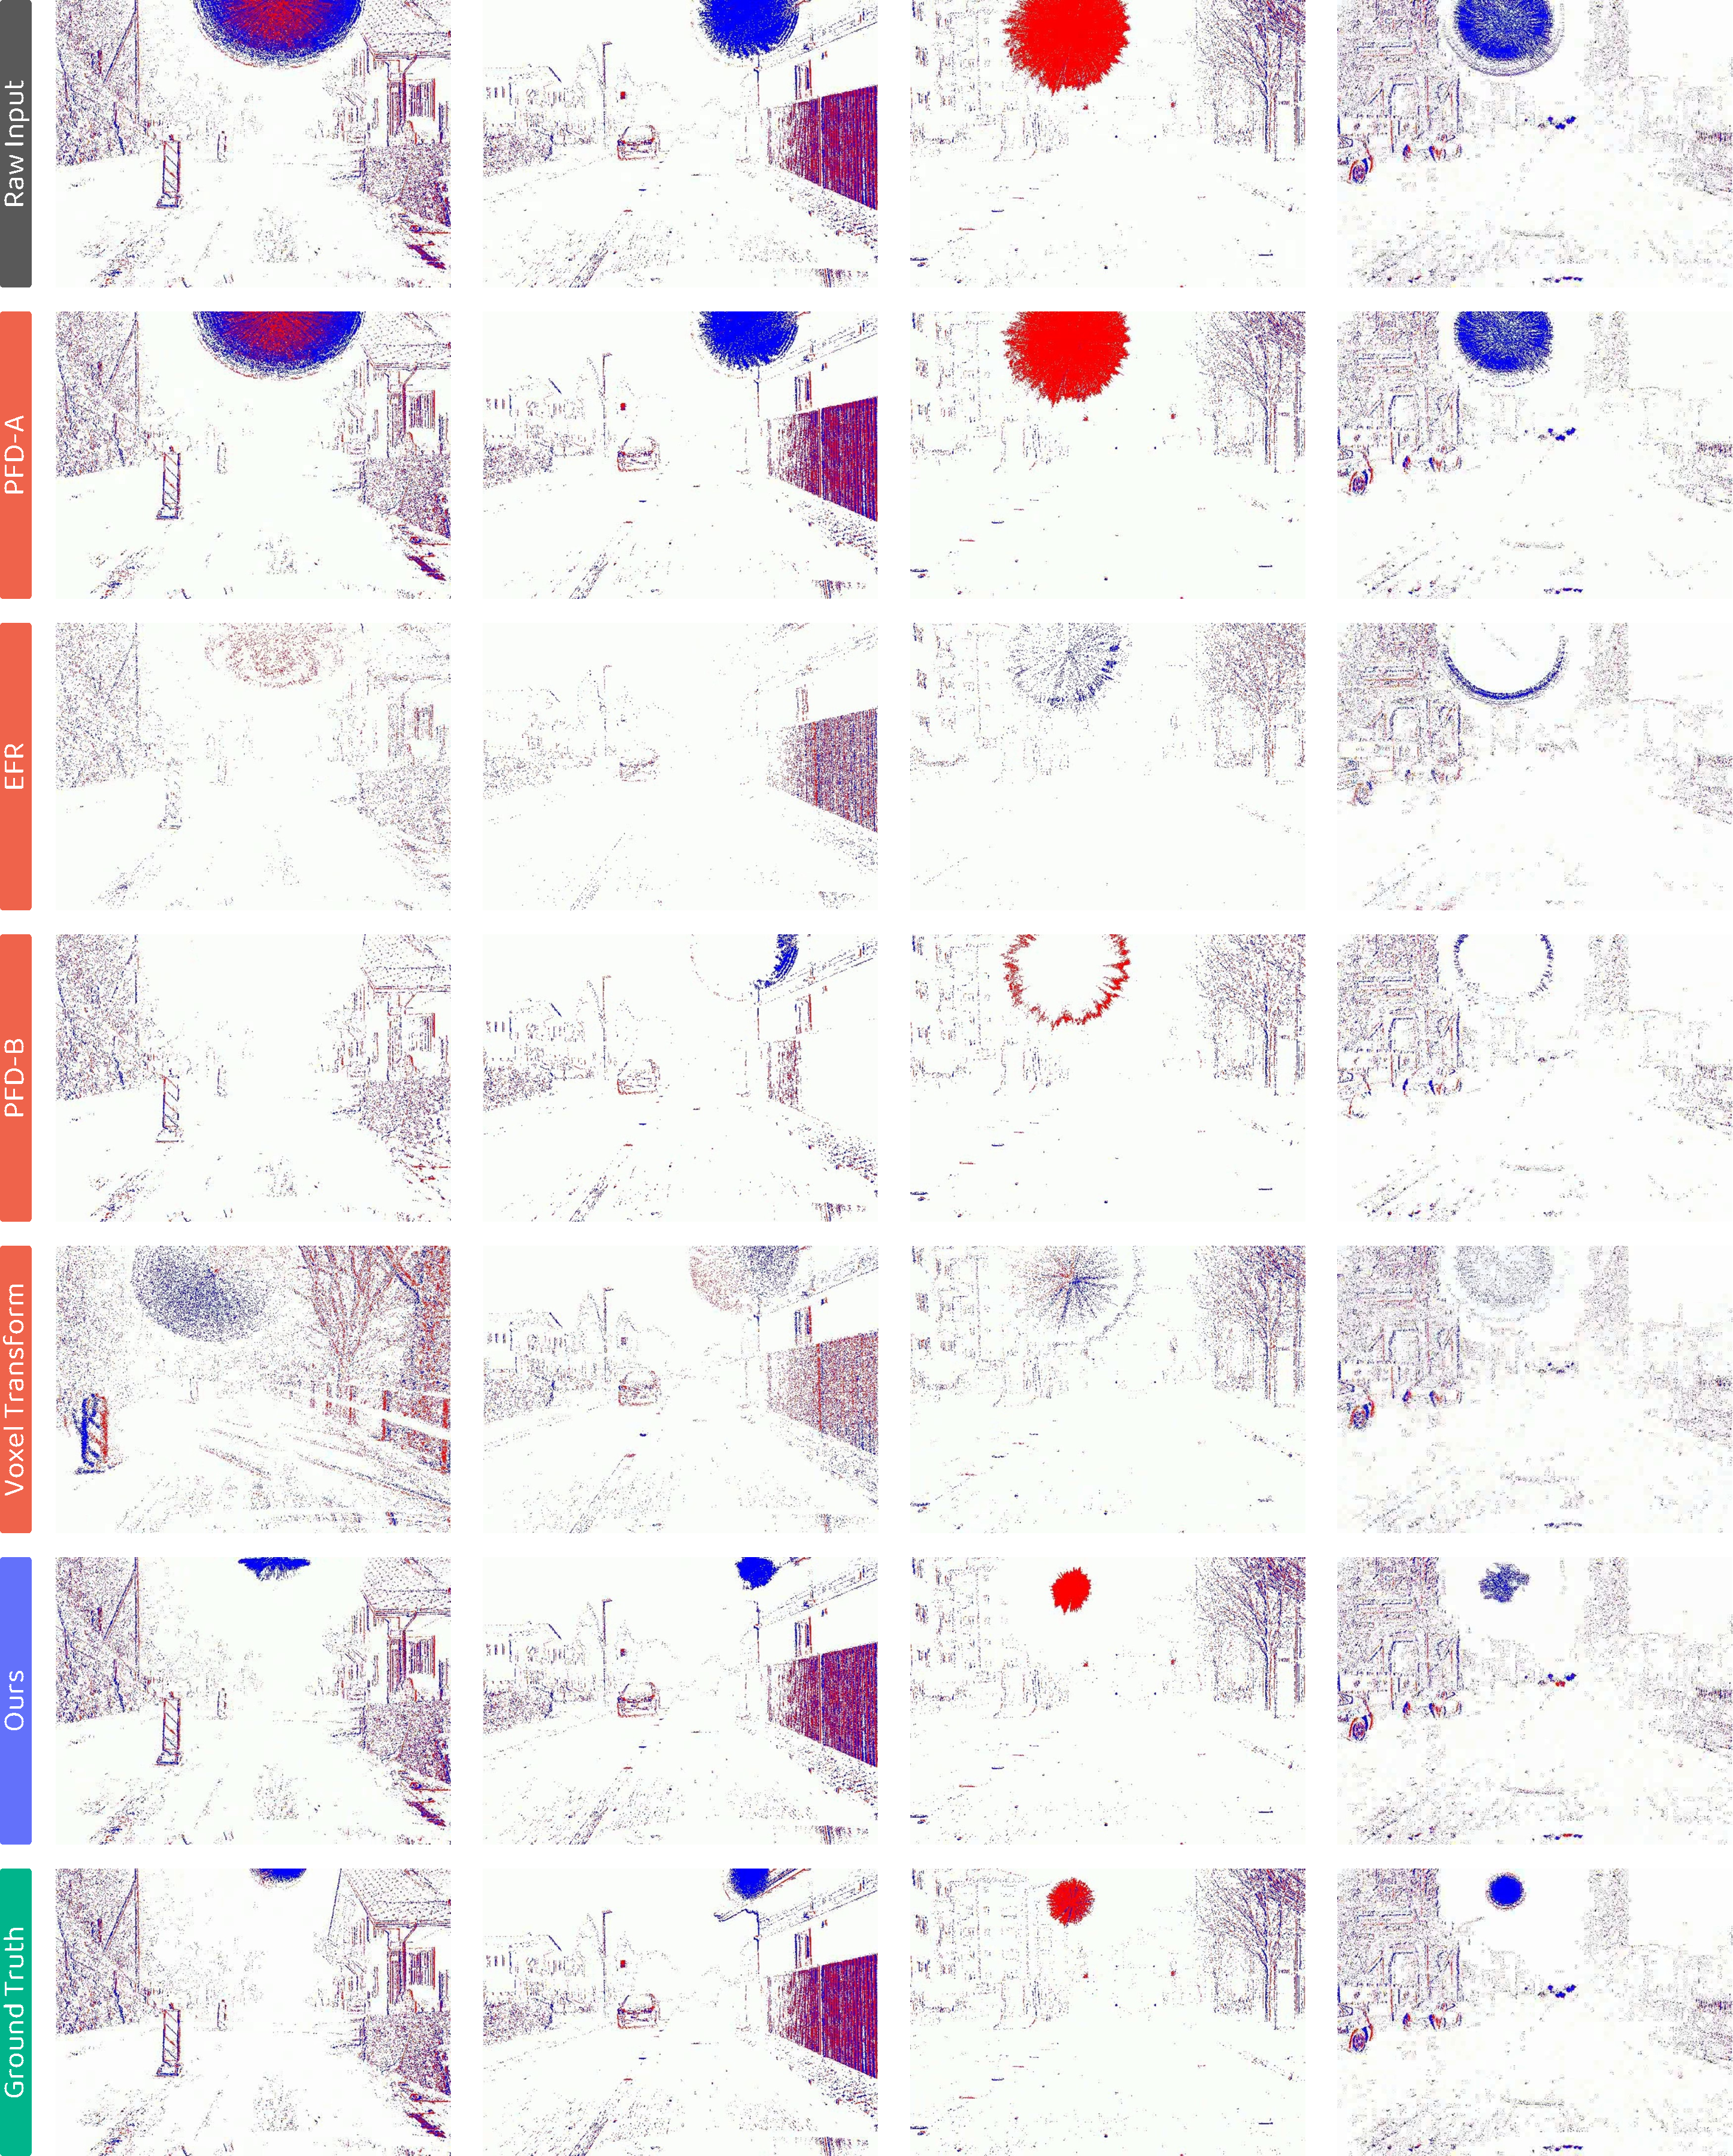
\includegraphics[width=\textwidth]{figures_supp/simu_R_supp_1.pdf}
    \caption{\textbf{Additional qualitative results on E-Flare2.7K.} Each row shows the output of a different method applied to the same flare-corrupted input. The bottom row displays the ground truth. Best viewed in color and zoomed in for details.}
    \label{APfig:supp_1}
\end{figure}

\begin{figure}[H]
    \centering
    \includegraphics[width=\textwidth]{figures_supp/simu_R_supp_2.pdf}
    \caption{\textbf{Additional qualitative results on E-Flare2.7K} (continued). Best viewed in color and zoomed in for details.}
    \label{APfig:supp_2}
\end{figure}

\subsection{Generalization to Extreme and Static Cases}

Fig.~\ref{APfig:supp_3} investigates model generalization under stress tests: extreme flare from light sources in close proximity, and \textbf{non-flickering (static) light sources} resembling continuous sunlight or stable DC lighting. Frequency-based baselines (\eg, EFR) rely on detecting temporal periodicity and fail completely on static flare. \textbf{E-DeflareNet}, by contrast, learns to recognize the intrinsic spatio-temporal morphology of flare rather than relying on temporal frequency, and remains stable and effective even in these challenging cases.

\begin{figure}[H]
    \centering
    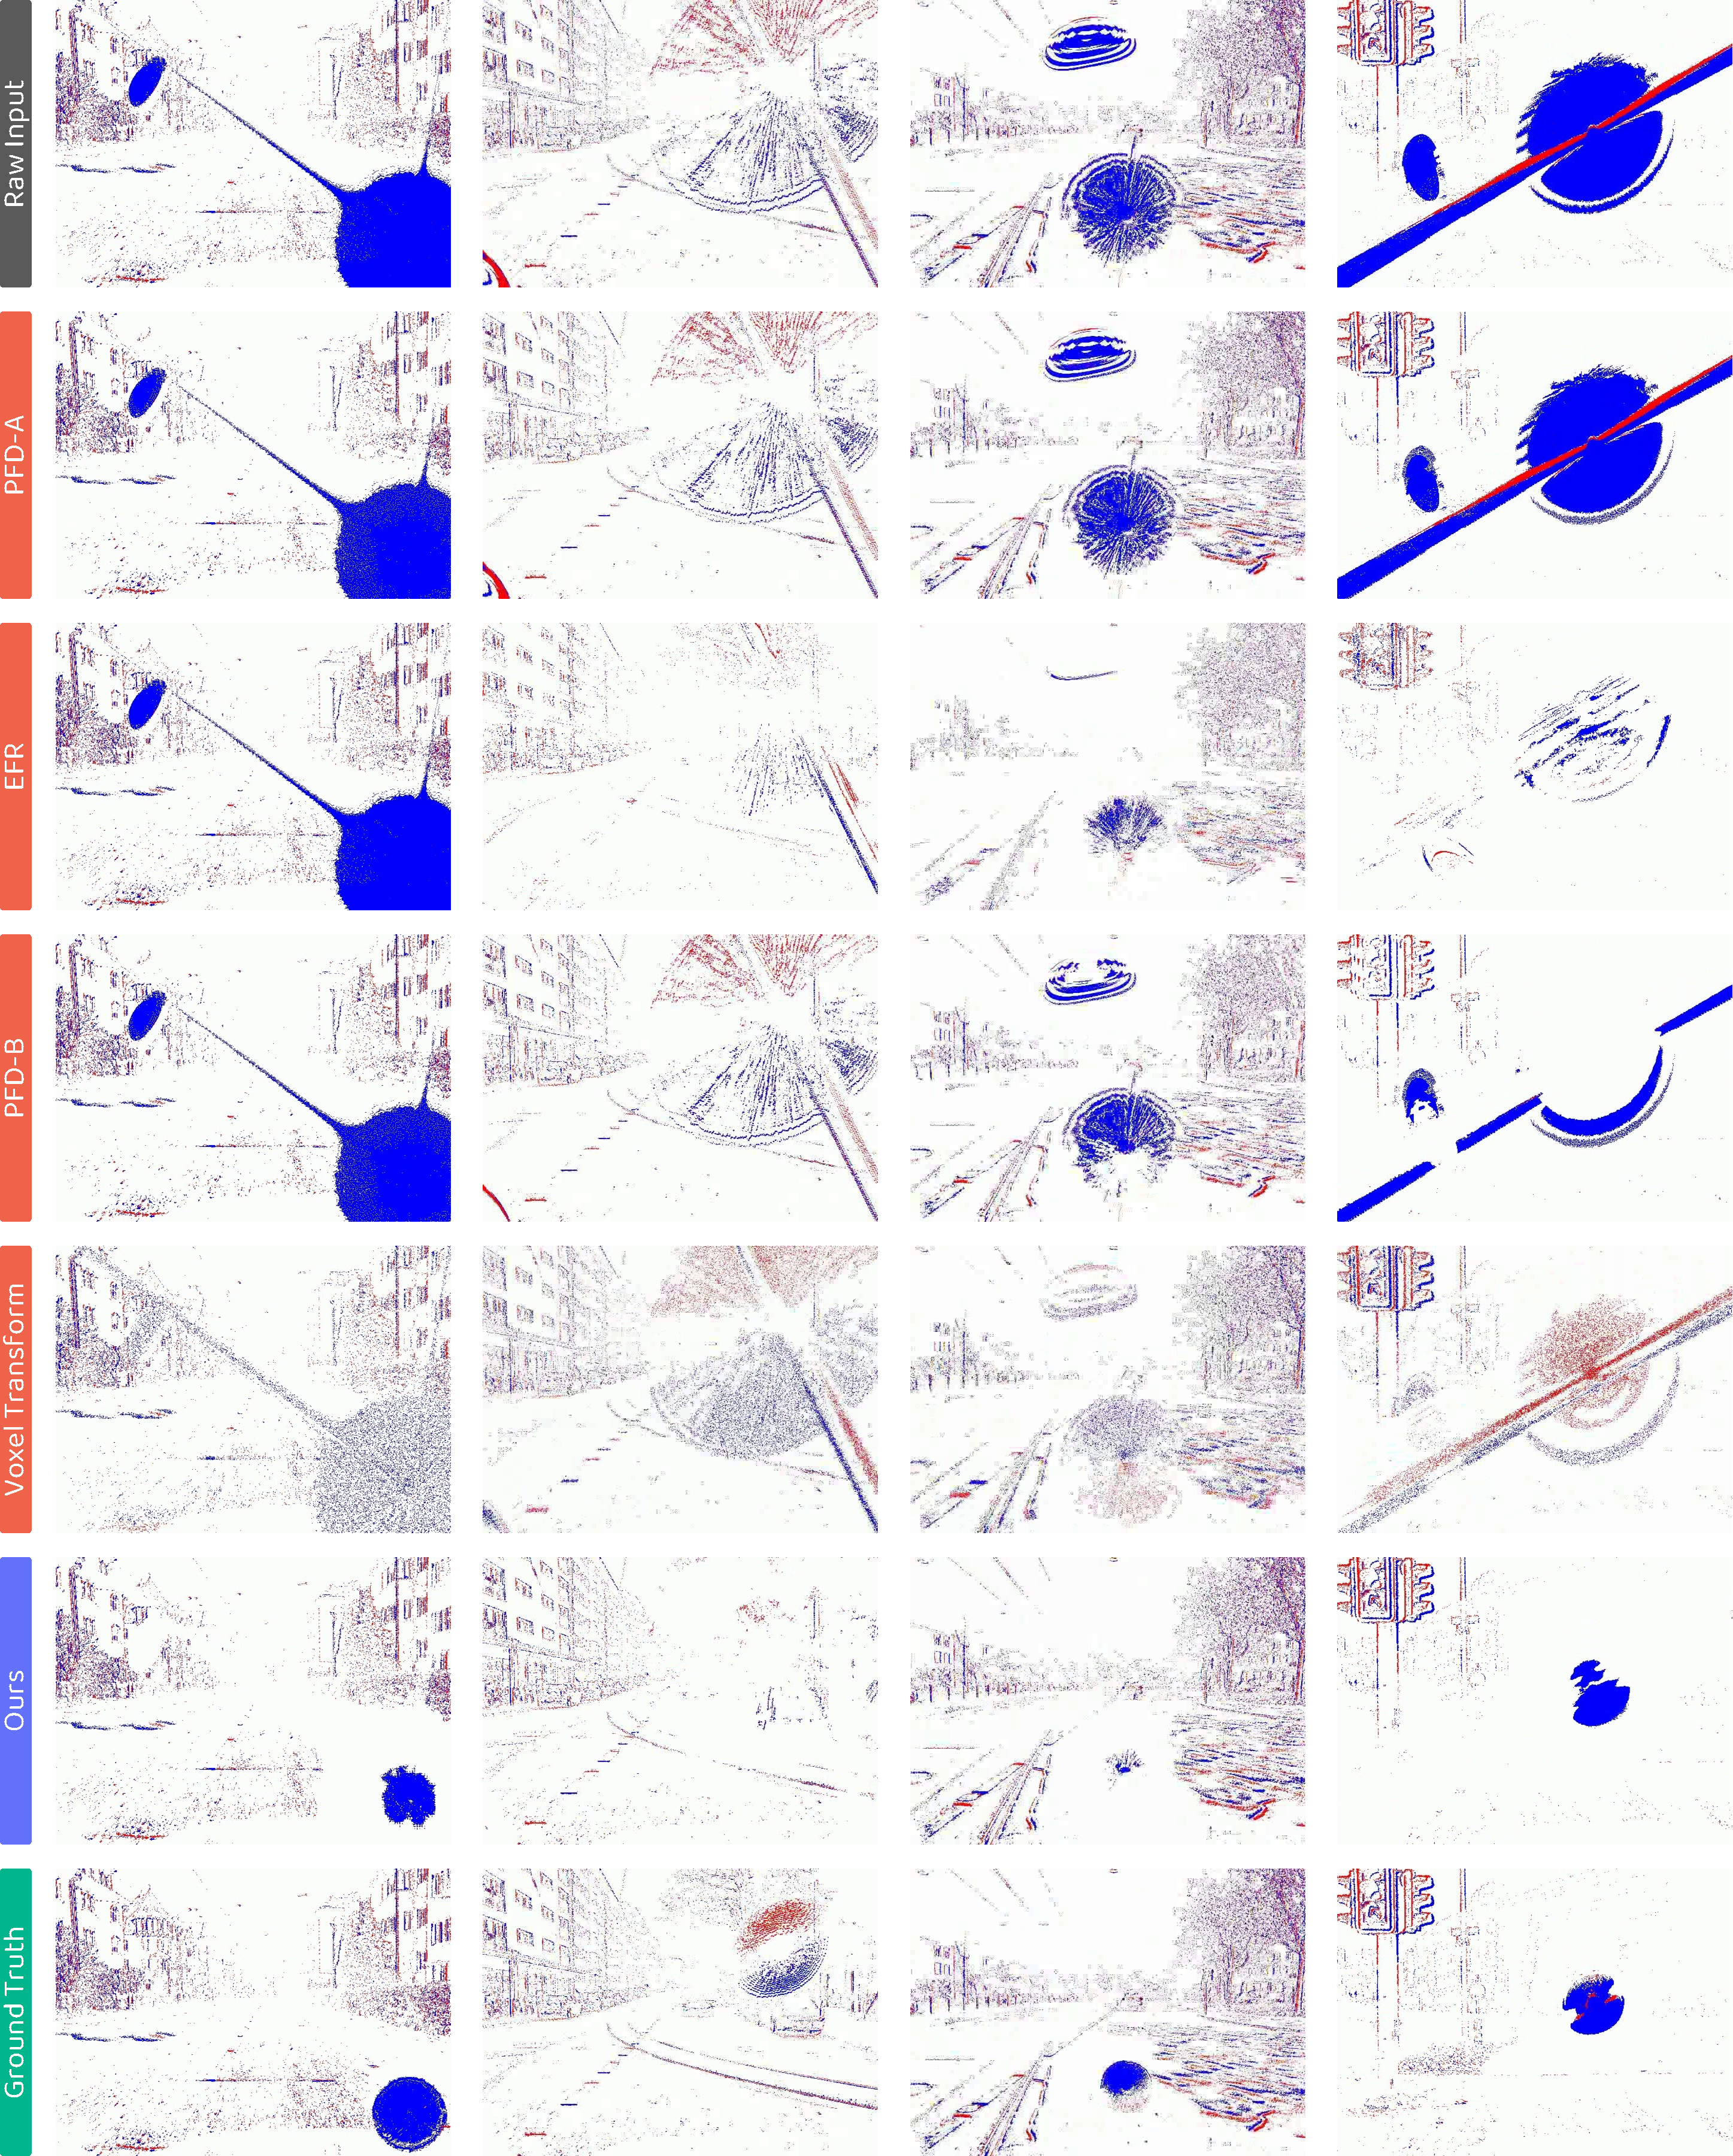
\includegraphics[width=\textwidth]{figures_supp/simu_R_supp_3.pdf}
    \caption{\textbf{Additional qualitative results on E-Flare2.7K} covering extreme and static-flare cases. Best viewed in color and zoomed in for details.}
    \label{APfig:supp_3}
\end{figure}

\subsection{Downstream Validation on 3D Reconstruction}
\label{app:3d_reconstruction}

We further evaluate \textbf{E-Deflare} on event-based 3D reconstruction. Since no standard benchmark with flare artifacts exists for this task, we synthesize paired event streams from the LEGO scene of NeRF-synthetic~\cite{mildenhall2021nerf}, following the event simulation protocol of PECS~\cite{han2024physical}. We reconstruct a 3D scene from each event stream using Event3DGS~\cite{han2024event}, render novel views, and compare them with the clean reference using background color normalization.

\begin{table}[H]
    \centering
    \caption{\textbf{Downstream task comparisons} for event-based 3D reconstruction. We use Event3DGS~\cite{han2024event} to reconstruct scenes and evaluate novel view synthesis. $\uparrow$: higher is better.}
    \label{tab:app_3dgs_quant}
    \small
    \resizebox{0.62\textwidth}{!}{%
    \begin{tabular}{r|c|ccc|c}
    \toprule
    \textbf{Metric} & \textcolor{gray}{Original} & EFR & PFD-A & PFD-B & \textbf{Ours}
    \\
    \midrule
    PSNR $\uparrow$ & \cellcolor{gray!20}\textcolor{gray}{$13.72$} & \cellcolor{ev_red!20}$13.74$ & $13.11$ & $13.32$ & \cellcolor{ev_blue!20}$\mathbf{13.78}$
    \\
    SSIM $\uparrow$ & \cellcolor{gray!20}\textcolor{gray}{$0.765$} & $0.741$ & \cellcolor{ev_red!20}$0.743$ & $0.734$ & \cellcolor{ev_blue!20}$\mathbf{0.792}$
    \\
    \bottomrule
    \end{tabular}}
\end{table}

\begin{figure}[H]
    \centering
    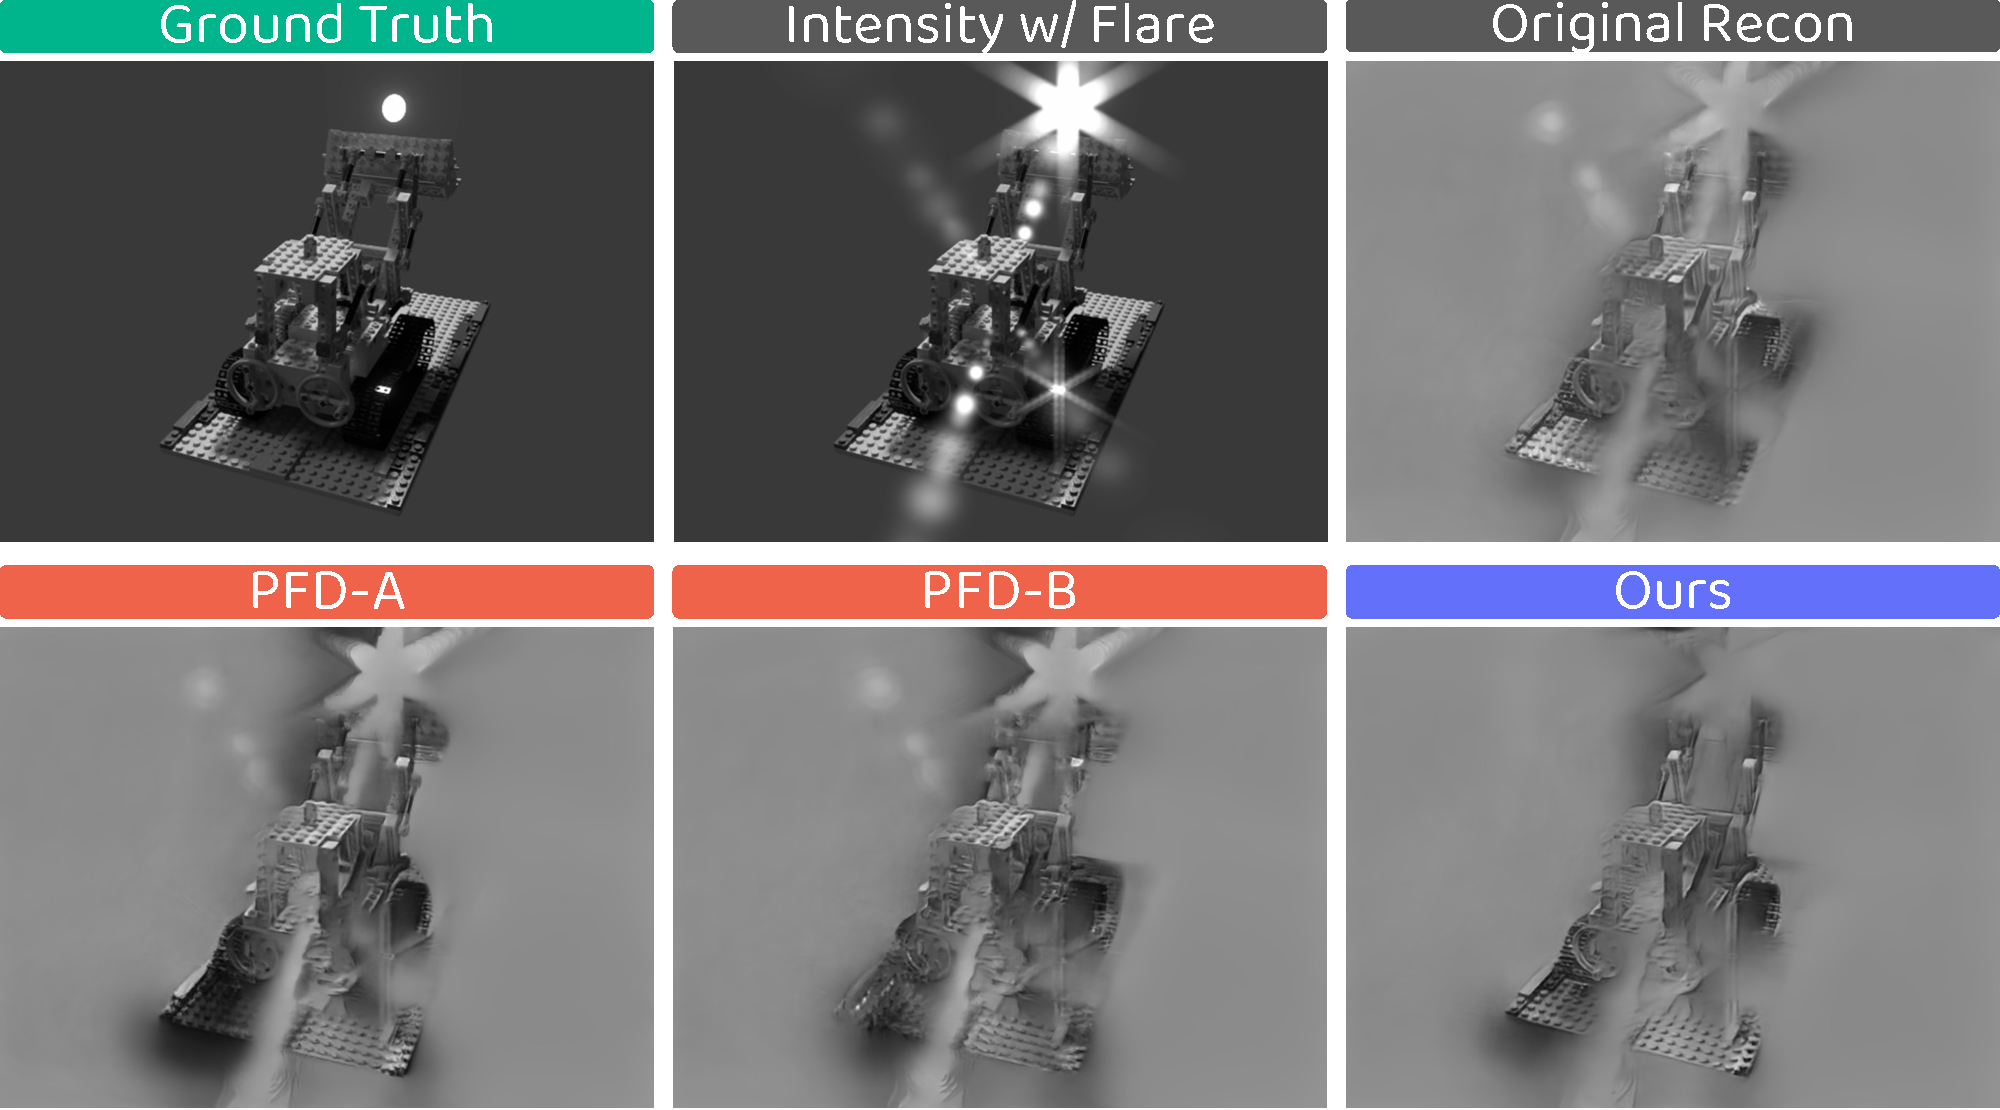
\includegraphics[width=0.72\textwidth]{figures/3D_reconstruction.pdf}
    \caption{\textbf{Downstream task comparisons} for event-based 3D reconstruction. We visualize rendered views from 3D scenes reconstructed using different de-flaring outputs.}
    \label{fig:app_3dgs_qual}
\end{figure}

The results show that naive de-flaring can harm 3D reconstruction, while our de-flared events provide a cleaner input and improve SSIM over the original flare-corrupted stream.

\subsection{Video Demonstrations}

Since event data is inherently temporal, static images cannot fully convey the dynamic quality of the restoration. We provide three video demonstrations attached to the supplementary material: \texttt{demo1.mp4} (E-Flare2.7K), \texttt{demo2.mp4} (E-Flare-R), and \texttt{demo3.mp4} (DSEC-Flare).


%% ============================================================
%% §F  Broader Impact & Limitations
%% ============================================================

\section{Broader Impact \& Limitations}
\label{app:impact_limitations}

In this section, we elaborate on the broader impact, societal influence, and potential limitations of the proposed approach.

\subsection{Broader Impact}

While this work focuses on lens flare removal, the theoretical framework and simulation-driven paradigm we propose have far-reaching implications for the field of neuromorphic vision.

\noindent\textbf{A Unified Framework for Additive Interference.}
Our derivation of the non-linear suppression mechanism provides a foundational tool for modeling any scenario where multiple light transport paths interact. This extends well beyond lens flare, offering a mathematically grounded blueprint for synthesizing data and training restoration networks for a wide class of previously intractable problems, including:

\begin{itemize}
    \item \emph{Reflections and Transparency:} Separating transmitted and reflected event streams in glass or water surfaces.
    \item \emph{Participating Media:} Modeling signal attenuation and scattering for perception in fog, rain, or underwater environments.
    \item \emph{Partial Occlusions:} Handling semi-transparent obstacles like smoke or foliage.
\end{itemize}

\noindent\textbf{Catalyzing Cross-Modal Synergy.}
Our work also hints at the immense potential of fusing event data with standard frame-based (RGB) modalities.

\begin{itemize}
    \item \emph{RGB-aided Event Restoration:} High-resolution RGB textures could serve as priors to guide the separation of flare from background events, improving the restoration of fine structural details that pure event-based methods might miss.
    \item \emph{Event-guided Image Enhancement:} Conversely, the high temporal resolution of event cameras makes them ideal for detecting the rapid onset and trajectory of dynamic flares. Our de-flaring capability could act as a robust attention mechanism, helping RGB image signal processors (ISPs) better localize and remove flare artifacts in conventional video.
\end{itemize}

\subsection{Societal Influence}
As a low-level enhancement module, \textbf{E-Deflare} poses no direct negative societal risks like labor displacement. Instead, it primarily benefits public safety by mitigating sensor blinding in autonomous vehicles during nighttime driving. Furthermore, our method adheres to privacy norms by recovering dynamic structures rather than sensitive static identities, maintaining the inherent privacy-preserving advantages of event cameras.

\subsection{Potential Limitations}

Despite the promising results, our current framework has limitations. First, the scale of our training data and model parameters is relatively modest; scaling these up could further enhance restoration fidelity, particularly in recovering background events under extreme suppression. Second, the computational cost of the 3D convolutional backbone poses a challenge for resource-constrained edge devices. Future work will focus on model compression and lightweight architectures to ensure real-time processing efficiency.


%% ============================================================
%% §G  Public Resources Used
%% ============================================================

\section{Public Resource Used}

In this section, we acknowledge the use of the following public resources during the course of this work.

\subsection{Public Datasets Used}
\begin{itemize}
    \item DSEC\footnote{\url{https://dsec.ifi.uzh.ch}} \dotfill CC BY-SA 4.0 License
    \item Flare7K++\footnote{\url{https://github.com/ykdai/Flare7K}} \dotfill S-Lab License 1.0
\end{itemize}

\subsection{Public Implementations Used}
\begin{itemize}
    \item SPADE-E2VID\footnote{\url{https://github.com/RodrigoGantier/SPADE_E2VID}} \dotfill Publicly Available
    \item Gaussian Splatting\footnote{\url{https://github.com/graphdeco-inria/gaussian-splatting}} \dotfill Inria / MPII License (Non-Commercial)
    \item pytorch-3dunet\footnote{\url{https://github.com/wolny/pytorch-3dunet}} \dotfill MIT License
    \item Flare Mania (Shadertoy)\footnote{\url{https://www.shadertoy.com/view/lsBGDK}} \dotfill CC BY-NC-SA 3.0
\end{itemize}
